%% LyX 2.3.4.2 created this file.  For more info, see http://www.lyx.org/.
%% Do not edit unless you really know what you are doing.
% \documentclass[english,dvipsnames,aspectratio=169]{beamer}
\documentclass[english,dvipsnames,aspectratio=169,handout]{beamer}
% \documentclass[english,dvipsnames,aspectratio=169,handout]{beamer}
\usepackage{mathptmx}
\usepackage{eulervm}
\usepackage[T1]{fontenc}
\usepackage[latin9]{inputenc}
\usepackage{babel}
\usepackage{amstext}
\usepackage{amssymb}
\usepackage{graphicx}
\usepackage{ifthen}
\usepackage{xcolor}
\usepackage{xspace}
\usepackage{tikz}
\usetikzlibrary{tikzmark}
\usetikzlibrary{calc}
\usepackage{pgfplots}
%\pgfplotsset{compat=1.17}
\usepackage{booktabs}
\usepackage{xpatch}
\usepackage{multirow}
\usepackage{colortbl}
\usepackage{pgfpages}
\usepackage{bbm}




\xpatchcmd{\itemize}
  {\def\makelabel}
  {\ifnum\@itemdepth=1\relax
     \setlength\itemsep{2ex}% separation for first level
   \else
     \ifnum\@itemdepth=2\relax
       \setlength\itemsep{1ex}% separation for second level
     \else
       \ifnum\@itemdepth=3\relax
         \setlength\itemsep{0.5ex}% separation for third level
   \fi\fi\fi\def\makelabel
  }
 {}
 {}

\ifx\hypersetup\undefined
  \AtBeginDocument{%
    \hypersetup{unicode=true,pdfusetitle,
 bookmarks=true,bookmarksnumbered=false,bookmarksopen=false,
 breaklinks=false,pdfborder={0 0 0},pdfborderstyle={},backref=false,colorlinks=true,
 allcolors=NYUPurple,urlcolor=LightPurple}
  }
\else
  \hypersetup{unicode=true,pdfusetitle,
 bookmarks=true,bookmarksnumbered=false,bookmarksopen=false,
 breaklinks=false,pdfborder={0 0 0},pdfborderstyle={},backref=false,colorlinks=true,
 allcolors=NYUPurple,urlcolor=LightPurple}
\fi

\makeatletter

%%%%%%%%%%%%%%%%%%%%%%%%%%%%%% LyX specific LaTeX commands.
%% Because html converters don't know tabularnewline
\providecommand{\tabularnewline}{\\}

%%%%%%%%%%%%%%%%%%%%%%%%%%%%%% Textclass specific LaTeX commands.
% this default might be overridden by plain title style
\newcommand\makebeamertitle{\frame{\maketitle}}%
% (ERT) argument for the TOC
\AtBeginDocument{%
  \let\origtableofcontents=\tableofcontents
  \def\tableofcontents{\@ifnextchar[{\origtableofcontents}{\gobbletableofcontents}}
  \def\gobbletableofcontents#1{\origtableofcontents}
}

%%%%%%%%%%%%%%%%%%%%%%%%%%%%%% User specified LaTeX commands.
\usetheme{CambridgeUS} 
\beamertemplatenavigationsymbolsempty


% Set Color ==============================
\definecolor{NYUPurple}{RGB}{87,6,140}
\definecolor{LightPurple}{RGB}{165,11,255}


\setbeamercolor{title}{fg=NYUPurple}
\setbeamercolor{frametitle}{fg=NYUPurple}

\setbeamercolor{background canvas}{fg=NYUPurple, bg=white}
\setbeamercolor{background}{fg=black, bg=NYUPurple}

\setbeamercolor{palette primary}{fg=black, bg=gray!30!white}
\setbeamercolor{palette secondary}{fg=black, bg=gray!20!white}
\setbeamercolor{palette tertiary}{fg=gray!20!white, bg=NYUPurple}

\setbeamertemplate{headline}{}
\setbeamerfont{itemize/enumerate body}{}
\setbeamerfont{itemize/enumerate subbody}{size=\normalsize}

\setbeamercolor{parttitle}{fg=NYUPurple}
\setbeamercolor{sectiontitle}{fg=NYUPurple}
\setbeamercolor{sectionname}{fg=NYUPurple}
\setbeamercolor{section page}{fg=NYUPurple}
%\setbeamercolor{description item}{fg=NYUPurple}
%\setbeamercolor{block title}{fg=NYUPurple}

\setbeamertemplate{blocks}[rounded][shadow=false]
\setbeamercolor{block body}{bg=normal text.bg!90!NYUPurple}
\setbeamercolor{block title}{bg=NYUPurple!30, fg=NYUPurple}



\AtBeginSection[]{
  \begin{frame}
  \vfill
  \centering
\setbeamercolor{section title}{fg=NYUPurple}
 \begin{beamercolorbox}[sep=8pt,center,shadow=true,rounded=true]{title}
    \usebeamerfont{title}\usebeamercolor[fg]{title}\insertsectionhead\par%
  \end{beamercolorbox}
  \vfill
  \end{frame}
}

\makeatother

\setlength{\parskip}{\medskipamount} 

\input ../macros

\begin{document}
\input ../rosenberg-macros

%\setbeameroption{show notes on second screen}

\title[CSCI-GA]{Neural Networks II: Deep Learning}
\author{Mengye Ren}
% \author{He He \\
% Slides based on Lecture
% \href{https://github.com/davidrosenberg/mlcourse/blob/gh-pages/Lectures/13a.k-means.pdf}{13a} from David Rosenberg's course materials (\url{https://github.com/davidrosenberg/mlcourse})
% }
\date{Nov 28, 2023}
\institute{NYU}

\makebeamertitle
\mode<article>{Just in article version}


\begin{frame}{Fully connected vs. locally connected}
\begin{itemize}
    \item So far we apply a layer where all output neurons are connected to all input neurons.
    \item In matrix form, $\mathbf{z} = W \mathbf{x}$.
    \item This is also called a fully connected layer or a dense layer or a linear layer.
    \pause
    \item For $200 \times 200$ image and 1000 hidden units, the matrix of a single layer will have 40M parameters!
\end{itemize}
\begin{center}
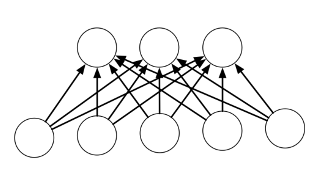
\includegraphics[width=0.34\textwidth]{figures/fully_connected.png}
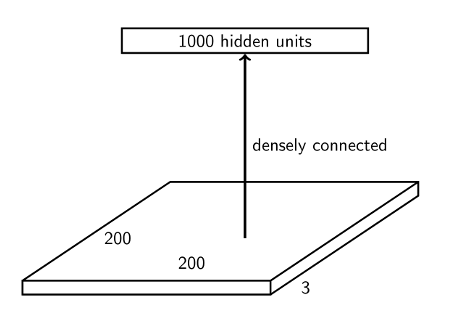
\includegraphics[width=0.34\textwidth]{figures/nn_1000_hidden.png}
\end{center}
\end{frame}
\begin{frame}{Fully connected vs. locally connected}
\begin{itemize}
    \item An alternative strategy is to use local connection.
    \item For neuron i, only connects to its neighborhood (e.g. [i+k, i-k])
    \item For images, we index neurons with three dimensions i, j, and c.
    \item i = vertical index, j = horizontal index, c = channel index.
\end{itemize}
\begin{center}
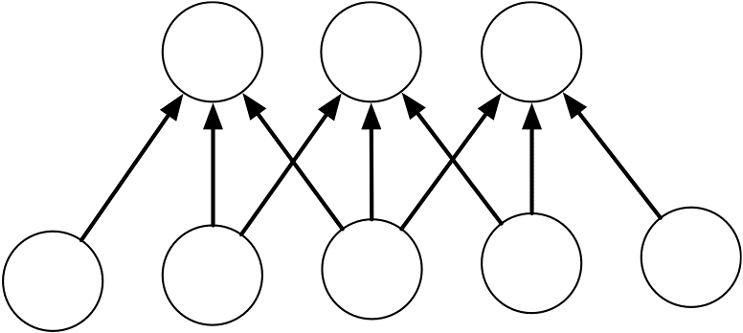
\includegraphics[width=0.3\textwidth]{figures/locally_connected.png}
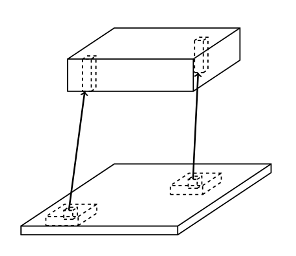
\includegraphics[width=0.3\textwidth]{figures/locally_connected_3d.png}
\end{center}
\end{frame}

\begin{frame}{Local connection patterns}
\begin{columns}
\begin{column}{0.65\textwidth}
\begin{itemize}
    \onslide<1->{\item The typical image input layer has 3 channels R G B for color or 1 channel for grayscale.
    \item The hidden layers may have $C$ channels, at each spatial location $(i, j)$.
    }
    \onslide<2->{
    \item Now each hidden neuron $z_{i,j,c}$ receives inputs from $x_{i \pm k, j \pm k, \cdot}$ 
    % - taking all the channels at neighboring spatial locations.
    \item $k$ is the ``kernel'' size - do not confuse with the other kernel we learned.
    \item $z_{i,j,c} = \sum_{i'\in[i\pm k], j' \in [j \pm k], c'} x_{i'j'c'} \textcolor{red}{w_{i, j, i'-i, j'-j, c',c}}$
    }
    \onslide<3->{
    \item The spatial awareness (receptive field) of the neighborhood grows bigger as we go deeper.
    }
\end{itemize}
\end{column}
\begin{column}{0.34\textwidth}
\begin{center}
\onslide<1->{
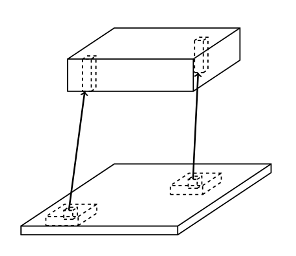
\includegraphics[width=0.8\textwidth]{figures/locally_connected_3d.png}
}
\end{center}
\end{column}
\end{columns}
\end{frame}

\begin{frame}{Weight sharing}
\begin{itemize}
\item Still a lot of weights: If we have 100 channels in the second layer, then $200 \times 200 \times 3 \times 100 = 12M$
\pause
\item Local information is the same regardless of the position of an element.
% \item E.g. A dog is a dog anywhere in an image.
\pause
\item Solution: We can tie the weights at different locations.
\end{itemize}
\begin{center}
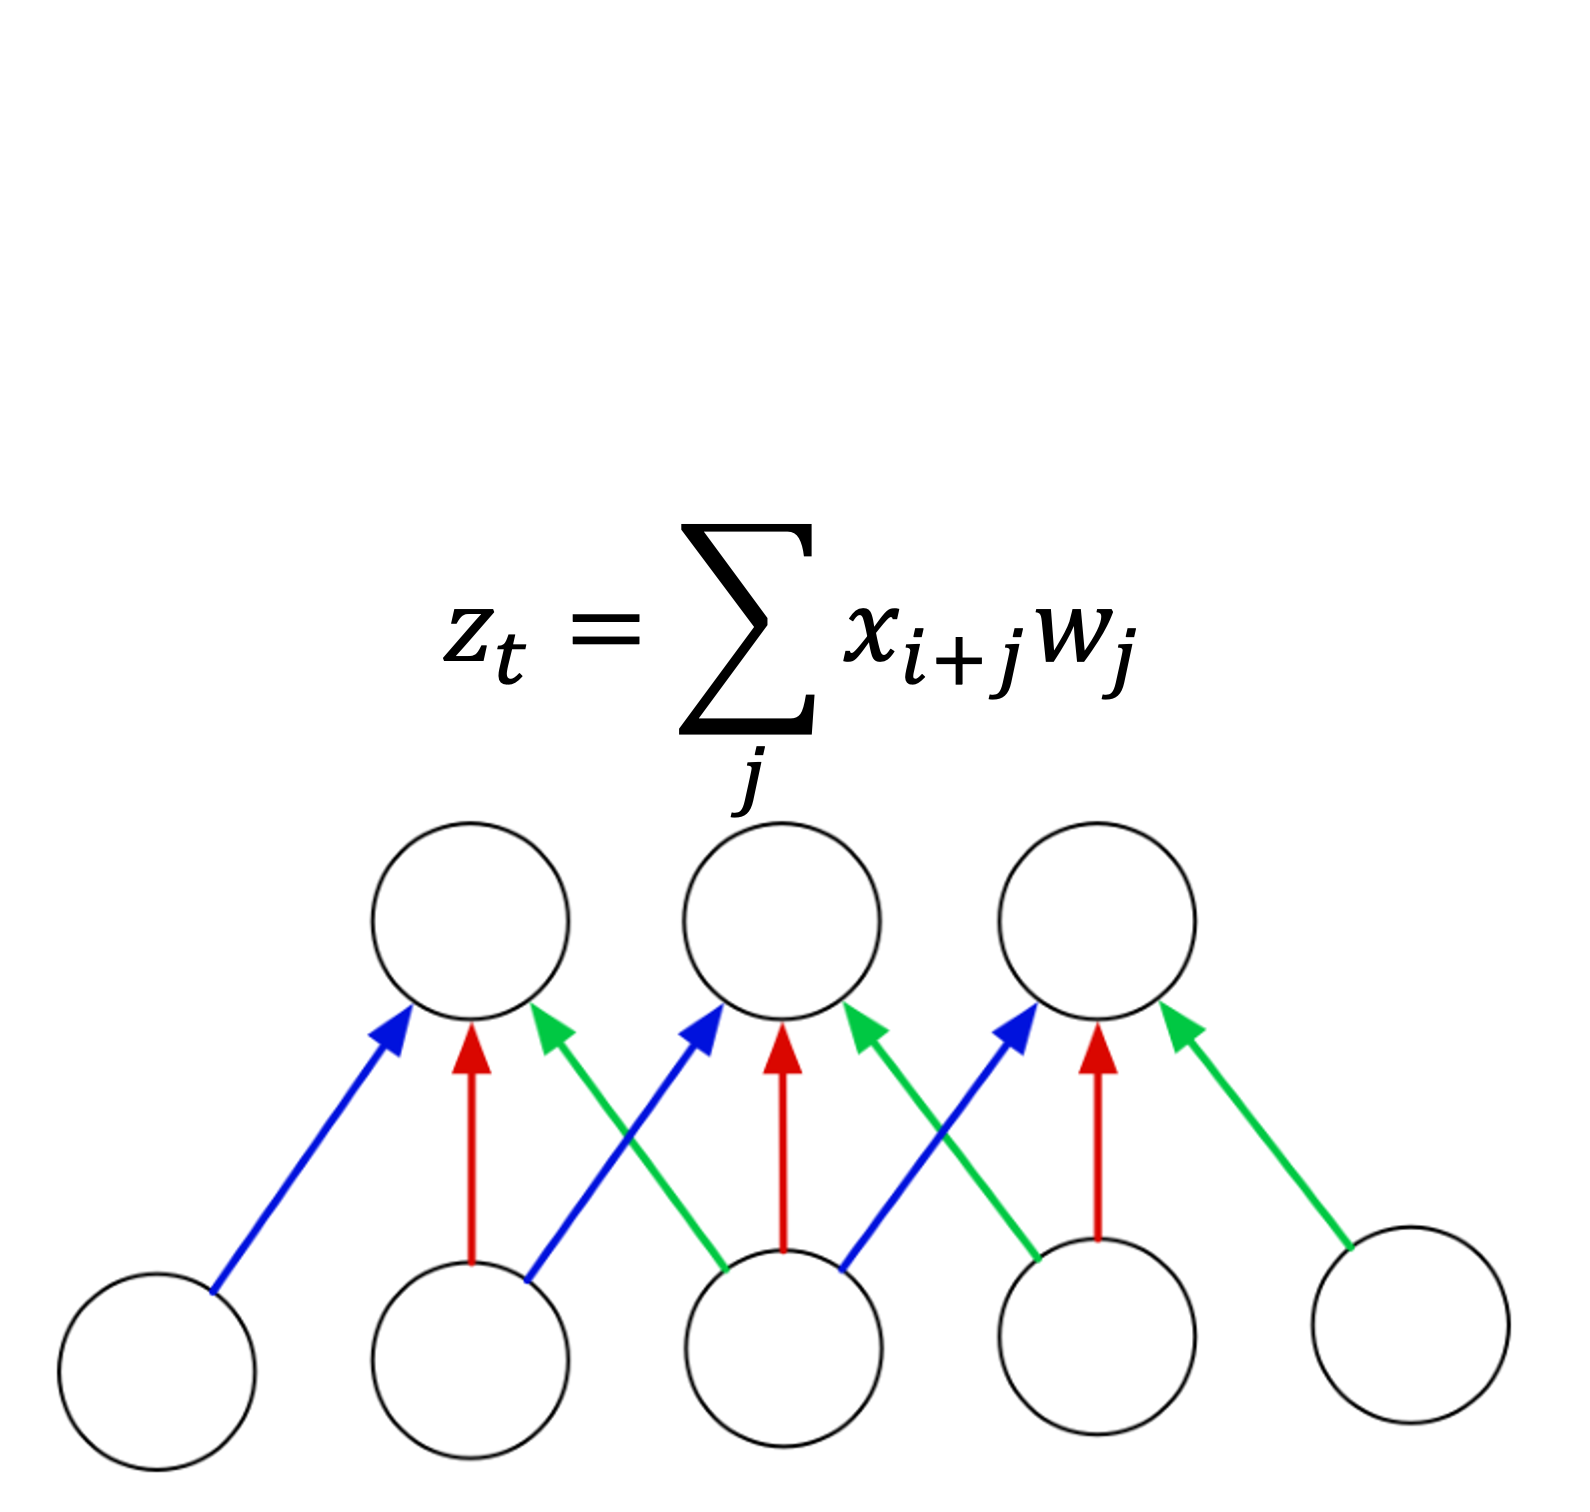
\includegraphics[width=0.3\textwidth,trim={0 0 0 6.2cm},clip]{figures/weight_share_2d.png}
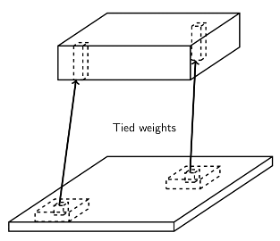
\includegraphics[width=0.3\textwidth]{figures/weight_share_3d.png}
\end{center}
\end{frame}

\begin{frame}{2D convolution}

\begin{columns}
\begin{column}{0.5\textwidth}
\begin{itemize}
    \item Using the same weight connections for each activation spatial location works like the ``filtering operation'' or ``convolution''
    \item The neighborhood window is the filter window.
    \item The weight connection is called ``convolution filter''
    \item $z_{i,j,c} = \sum_{i'\in[i\pm k], j' \in [j \pm k], c'} x_{i'j'c'} \textcolor{red}{w_{i-i', j-j', c',c}}$
\end{itemize}
\end{column}
\begin{column}{0.5\textwidth}
\begin{center}
\includegraphics<1>[width=0.8\textwidth]{figures/2d_conv/frame_0.png}
\includegraphics<2>[width=0.8\textwidth]{figures/2d_conv/frame_1.png}
\includegraphics<3>[width=0.8\textwidth]{figures/2d_conv/frame_2.png}
\includegraphics<4>[width=0.8\textwidth]{figures/2d_conv/frame_3.png}
\includegraphics<5>[width=0.8\textwidth]{figures/2d_conv/frame_4.png}
\includegraphics<6>[width=0.8\textwidth]{figures/2d_conv/frame_5.png}
\includegraphics<7>[width=0.8\textwidth]{figures/2d_conv/frame_6.png}
\includegraphics<8>[width=0.8\textwidth]{figures/2d_conv/frame_7.png}
\includegraphics<9>[width=0.8\textwidth]{figures/2d_conv/frame_8.png}
\end{center}
\end{column}
\end{columns}
\end{frame}

\begin{frame}{Pooling}
\begin{columns}
\begin{column}{0.5\textwidth}
\begin{itemize}
    \item Need to summarize global information more efficiently.
    \item Pooling reduces image / activation dimensions.
    \item Max-pooling or average-pooling
    \onslide<2->{
    \item You can also perform a ``strided'' convolution by jumping multiple steps.
    }
\end{itemize}
\end{column}
\begin{column}{0.5\textwidth}
\begin{center}
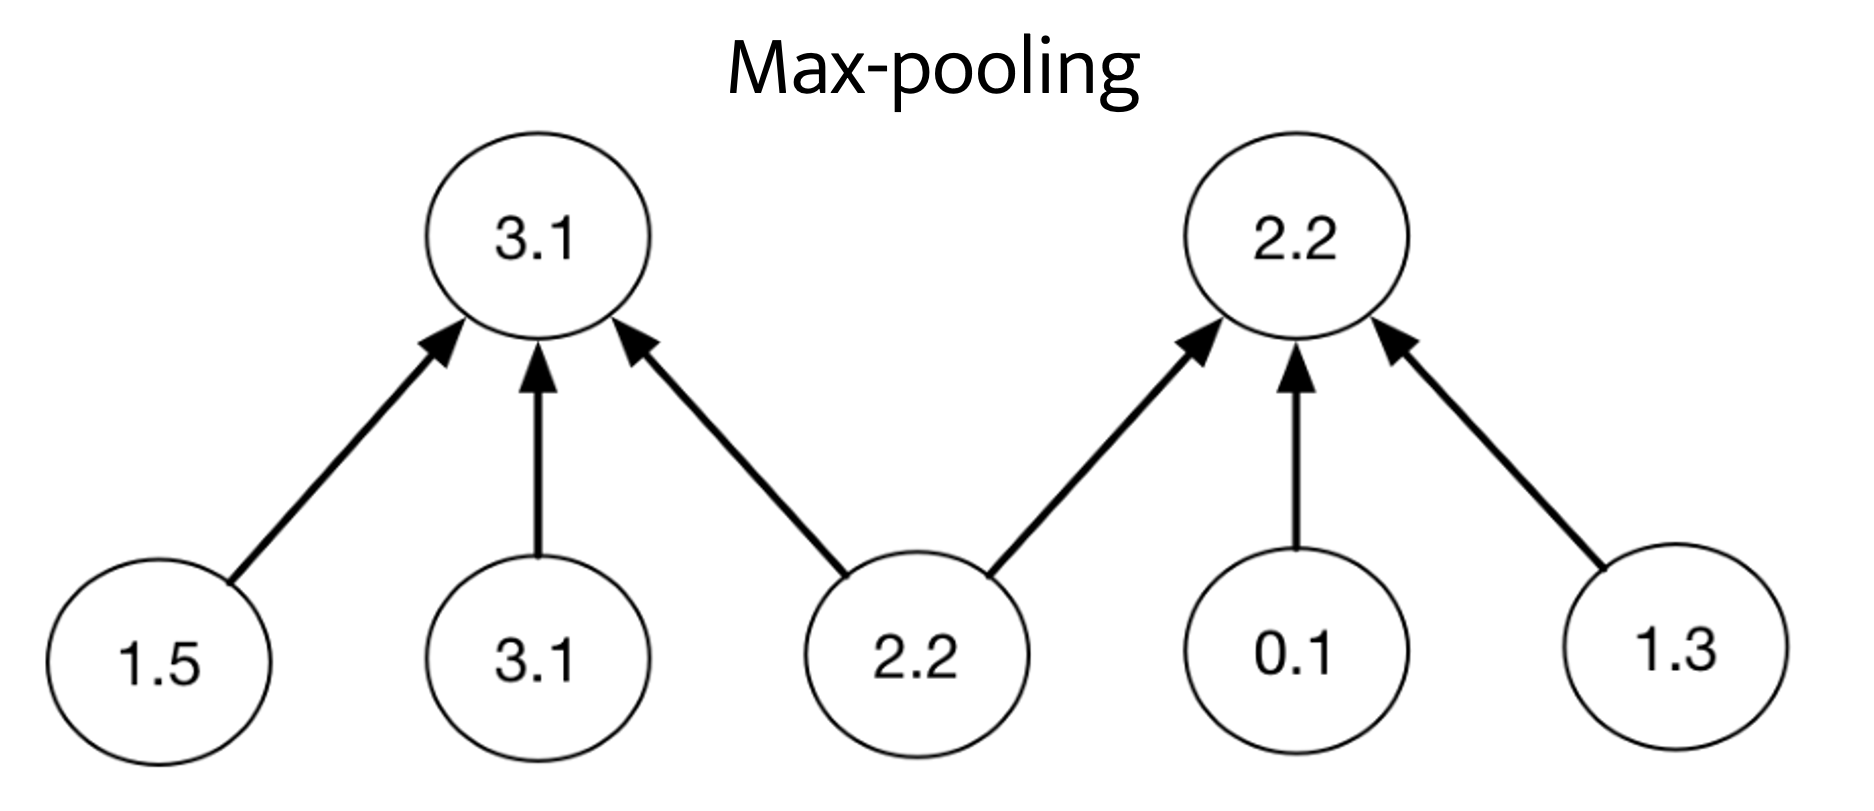
\includegraphics[width=0.8\textwidth]{figures/maxpooling.png}
\includegraphics<2>[width=0.5\textwidth]{figures/stride2_conv/frame_0.png}
\includegraphics<3>[width=0.5\textwidth]{figures/stride2_conv/frame_1.png}
\includegraphics<4>[width=0.5\textwidth]{figures/stride2_conv/frame_2.png}
\includegraphics<5>[width=0.5\textwidth]{figures/stride2_conv/frame_3.png}
\end{center}
\end{column}
\end{columns}
\end{frame}

\begin{frame}{Assembling together: LeNet}
\begin{center}
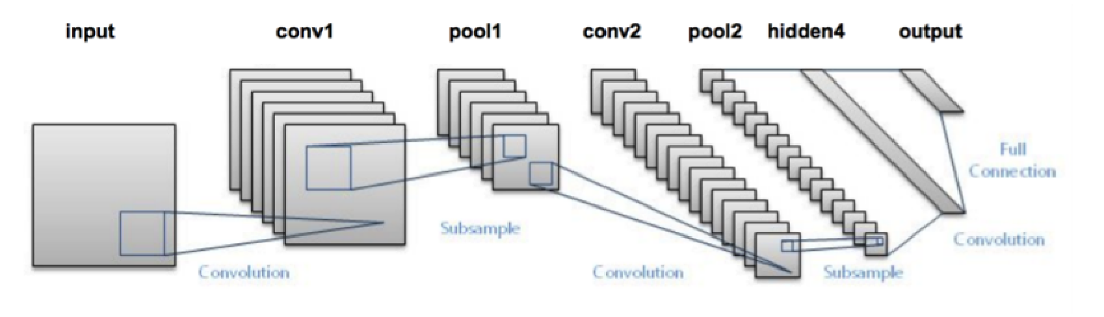
\includegraphics[width=0.8\textwidth]{figures/lenet2.png}
\end{center}
\begin{itemize}
    \item Used by USPS to read post code in the 90s.
\end{itemize}
\end{frame}

\begin{frame}{Historical development}
\begin{itemize}
    \item LeNet has worked and being put to practice in the 1990s.
    \pause
    \item Neural networks for images start to dominate in the last 10 years (starting 2012) for understanding general high resolution natural images.
    \pause
    \item During the years:
    \begin{itemize}
        \item Neural networks were difficult to work
        \item People focused on feature engineering
        \item Then apply SVM or random forest (e.g. AdaBoost face detector)
        \item What has changed?
    \end{itemize}
\end{itemize}
\end{frame}

\section{Gradient learning conditioning}
\begin{frame}{Optimization challenges}
\begin{itemize}
    \item Larger images require deeper networks (more stages of processing at different resolutions)
    \item Optimizing deeper layers of networks is not trivial.
    \item Loss often stalls or blows up.
    \item Why?
    \pause
    \begin{itemize}
        \item Backpropagation: multiplying the Jacobian $\frac{\partial y}{\partial x}$ by each layer.
        \item If the maximum singular value of each layer of Jacobian is less than 1: then the gradient will converge to 0 with more layers.
        \item If the greater than 1: then the gradient will explode with more layers.
        \item The bottom (input) layer may get 0 or infinite gradients.
    \end{itemize}
\end{itemize}
\end{frame}

\begin{frame}{Weight initialization}
\begin{itemize}
    \item Even with a few layers (>3), optimization is still hard.
    \item If weight initialization is bad (too small or too big), then optimization is hard to kick off.
    \item Consider the distribution of whole dataset in the activation space.
    % \item Pre-activation: $z=Wx$; Post-activation: $h=f(z)$
    \begin{itemize}
        % \item The mean of the pre-activations should be zero.
        \item Intuition: upon initialization, the variance of the activations should stay the same across every layer.
    \end{itemize}
\end{itemize}
\end{frame}

\begin{frame}{Kaiming Initialization}
\begin{itemize}
    \item Suppose each neuron and weight connection are sampling from a random distribution.
    \pause
    \item At $l$-th layer, $Var[z_l] = n_l Var[w_l x_l]$ ($n_l$ = num. input neurons to $l$-th layer)
    \pause
    \item If we suppose that ReLU is used as the activation, and $w_l$ is symmetric and zero-mean, $x_{l+1} = \frac{1}{2} Var[z_{l}]$.
    \pause
    \item Putting altogether, $x_{l+1} = \frac{1}{2} n_l Var[w_{l}] Var[x_l]$.
    \pause
    \item To make the variance constant, we need $\frac{1}{2} n_l Var[w_{l}] = 1$, $Std[w_{l}] = \sqrt{2/n_l}$\footnote{He et al. Delving Deep into Rectifiers: Surpassing Human-Level Performance on ImageNet. ICCV, 2015.}.
\end{itemize}
\end{frame}

\begin{frame}{Activation functions}
\begin{itemize}
    \item ReLU was proposed in 2009-2010\footnote{Jarrett et al. What is the Best Multi-Stage Architecture for Object Recognition? ICCV, 2009.}\footnote{Nair \& Hinton/ Rectified Linear Units Improve Restricted Boltzmann Machines. ICML, 2010.}, and was successfully used in AlexNet in 2012\footnote{Krizhevsky et al. 
ImageNet Classification with Deep Convolutional Neural Networks. NIPS, 2012.}.
    \item Address the vanishing gradient issue in activations, comparing to sigmoid or tanh.
    % \item More variants of activation function in the past decade.
\end{itemize}
\begin{center}
    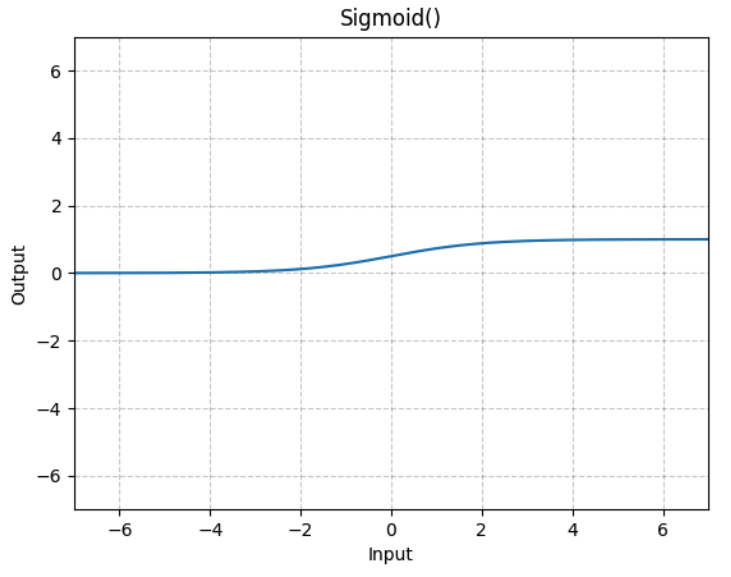
\includegraphics[width=0.17\textwidth]{figures/sigmoid.png}
    \quad
    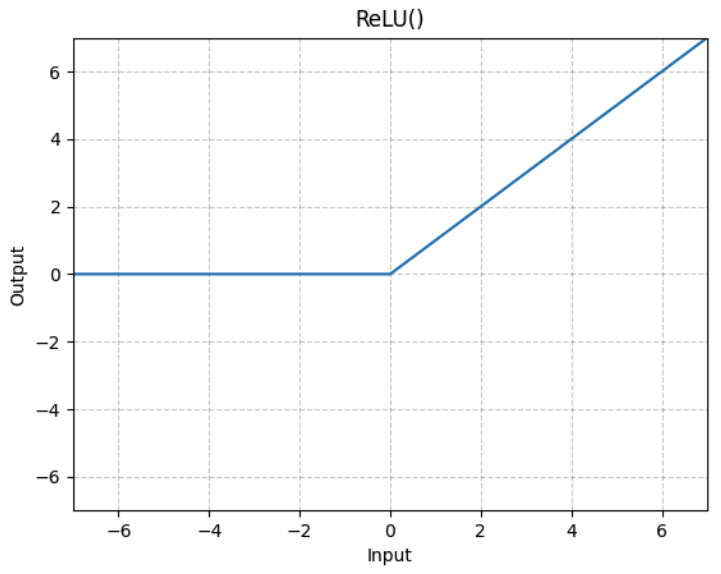
\includegraphics[width=0.17\textwidth]{figures/relu.png}
    \quad
    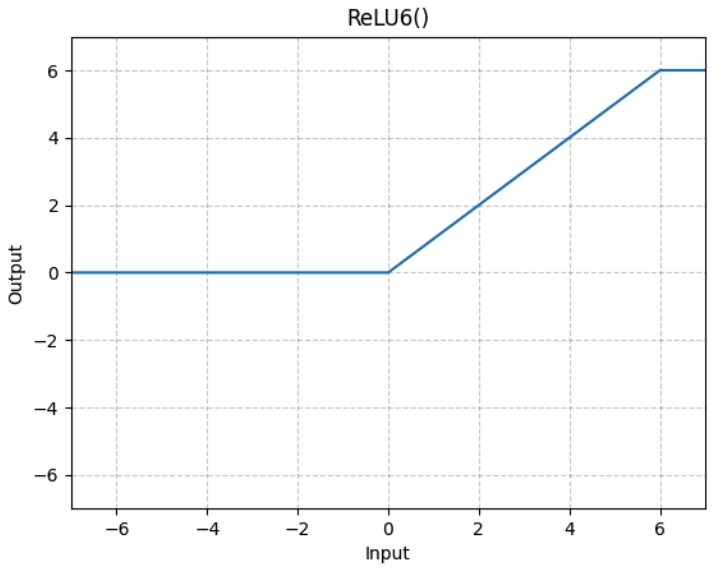
\includegraphics[width=0.17\textwidth]{figures/relu6.png}

    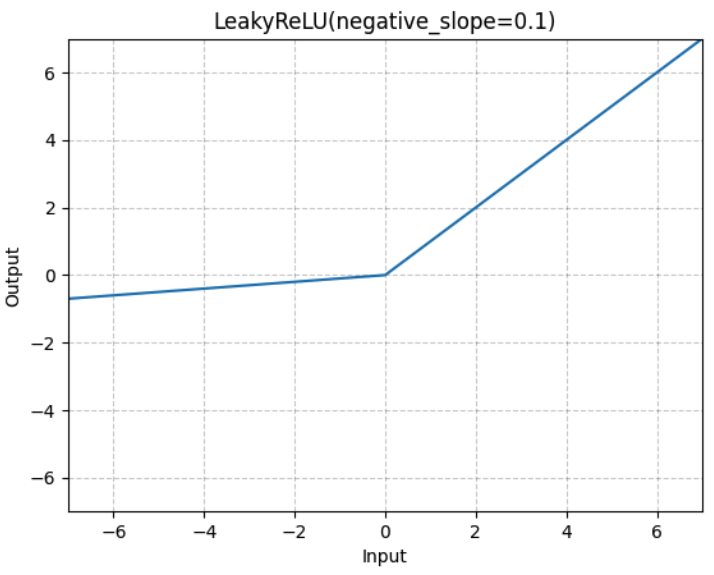
\includegraphics[width=0.17\textwidth]{figures/leaky_relu.png}
    \quad
    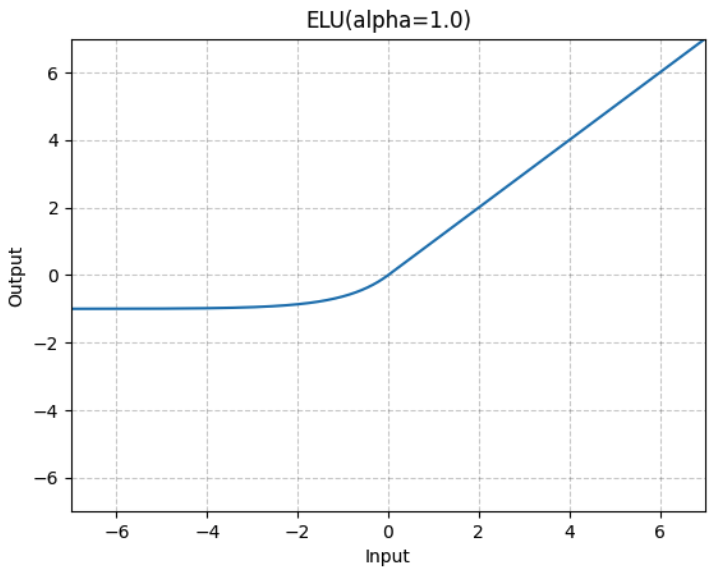
\includegraphics[width=0.17\textwidth]{figures/elu.png}
    \quad
    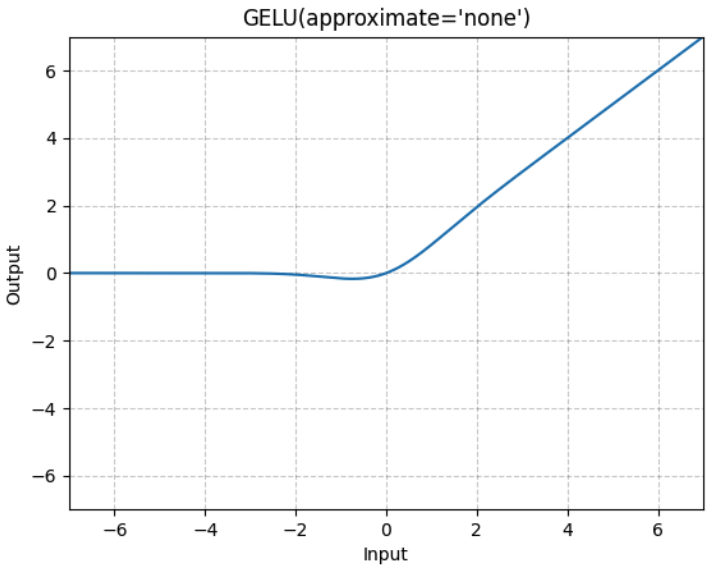
\includegraphics[width=0.17\textwidth]{figures/gelu.png}
\end{center}
\end{frame}

\begin{frame}{SGD Learning Rate}
  \begin{itemize}
    \item In stochastic training, the learning rate also influences the \alert{fluctuations} due to the stochasticity of the gradients.
    \item Typical strategy:
      \begin{itemize}
        \item Use a large learning rate early in training so you can get close to the optimum
        \item Gradually decay the learning rate to reduce the fluctuations
      \end{itemize}
  \end{itemize}
\end{frame}

\begin{frame}{Learning Rate Decay}
    \begin{itemize}
      \item We also need to be aware about the impact of learning rate due to the stochasticity.
    \end{itemize}
    \begin{center}
      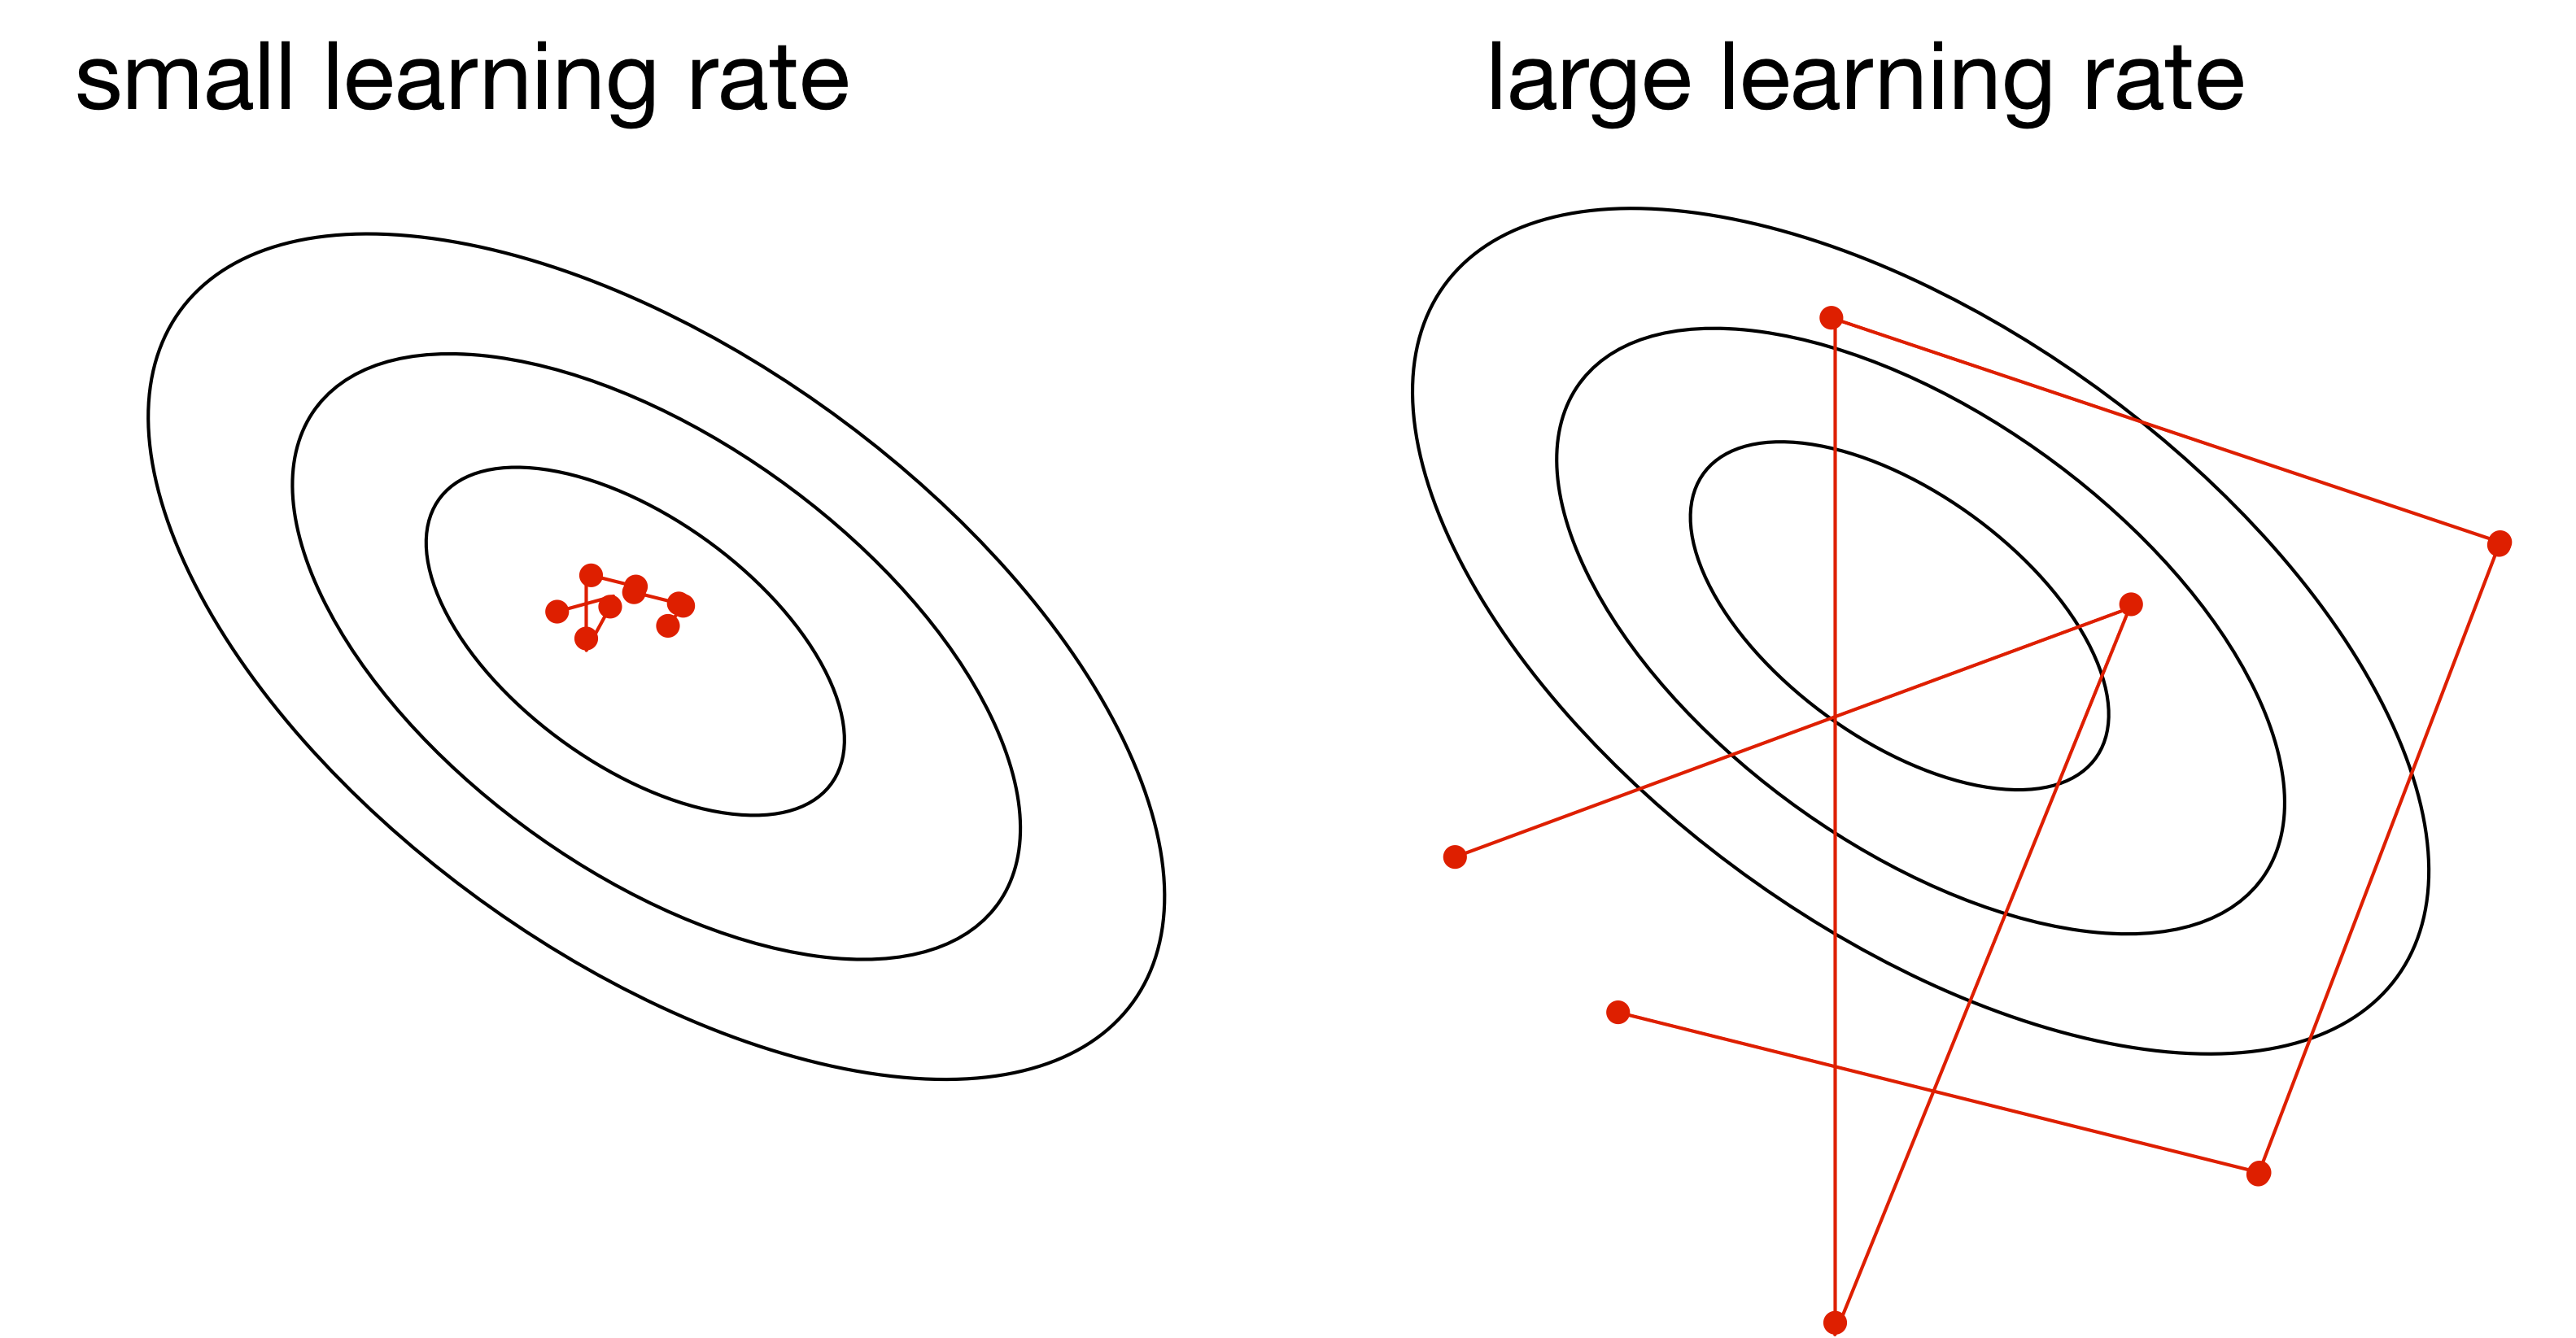
\includegraphics[width=0.3\textwidth]{figures/fluctuations.png}
    \end{center}
    \begin{center}
      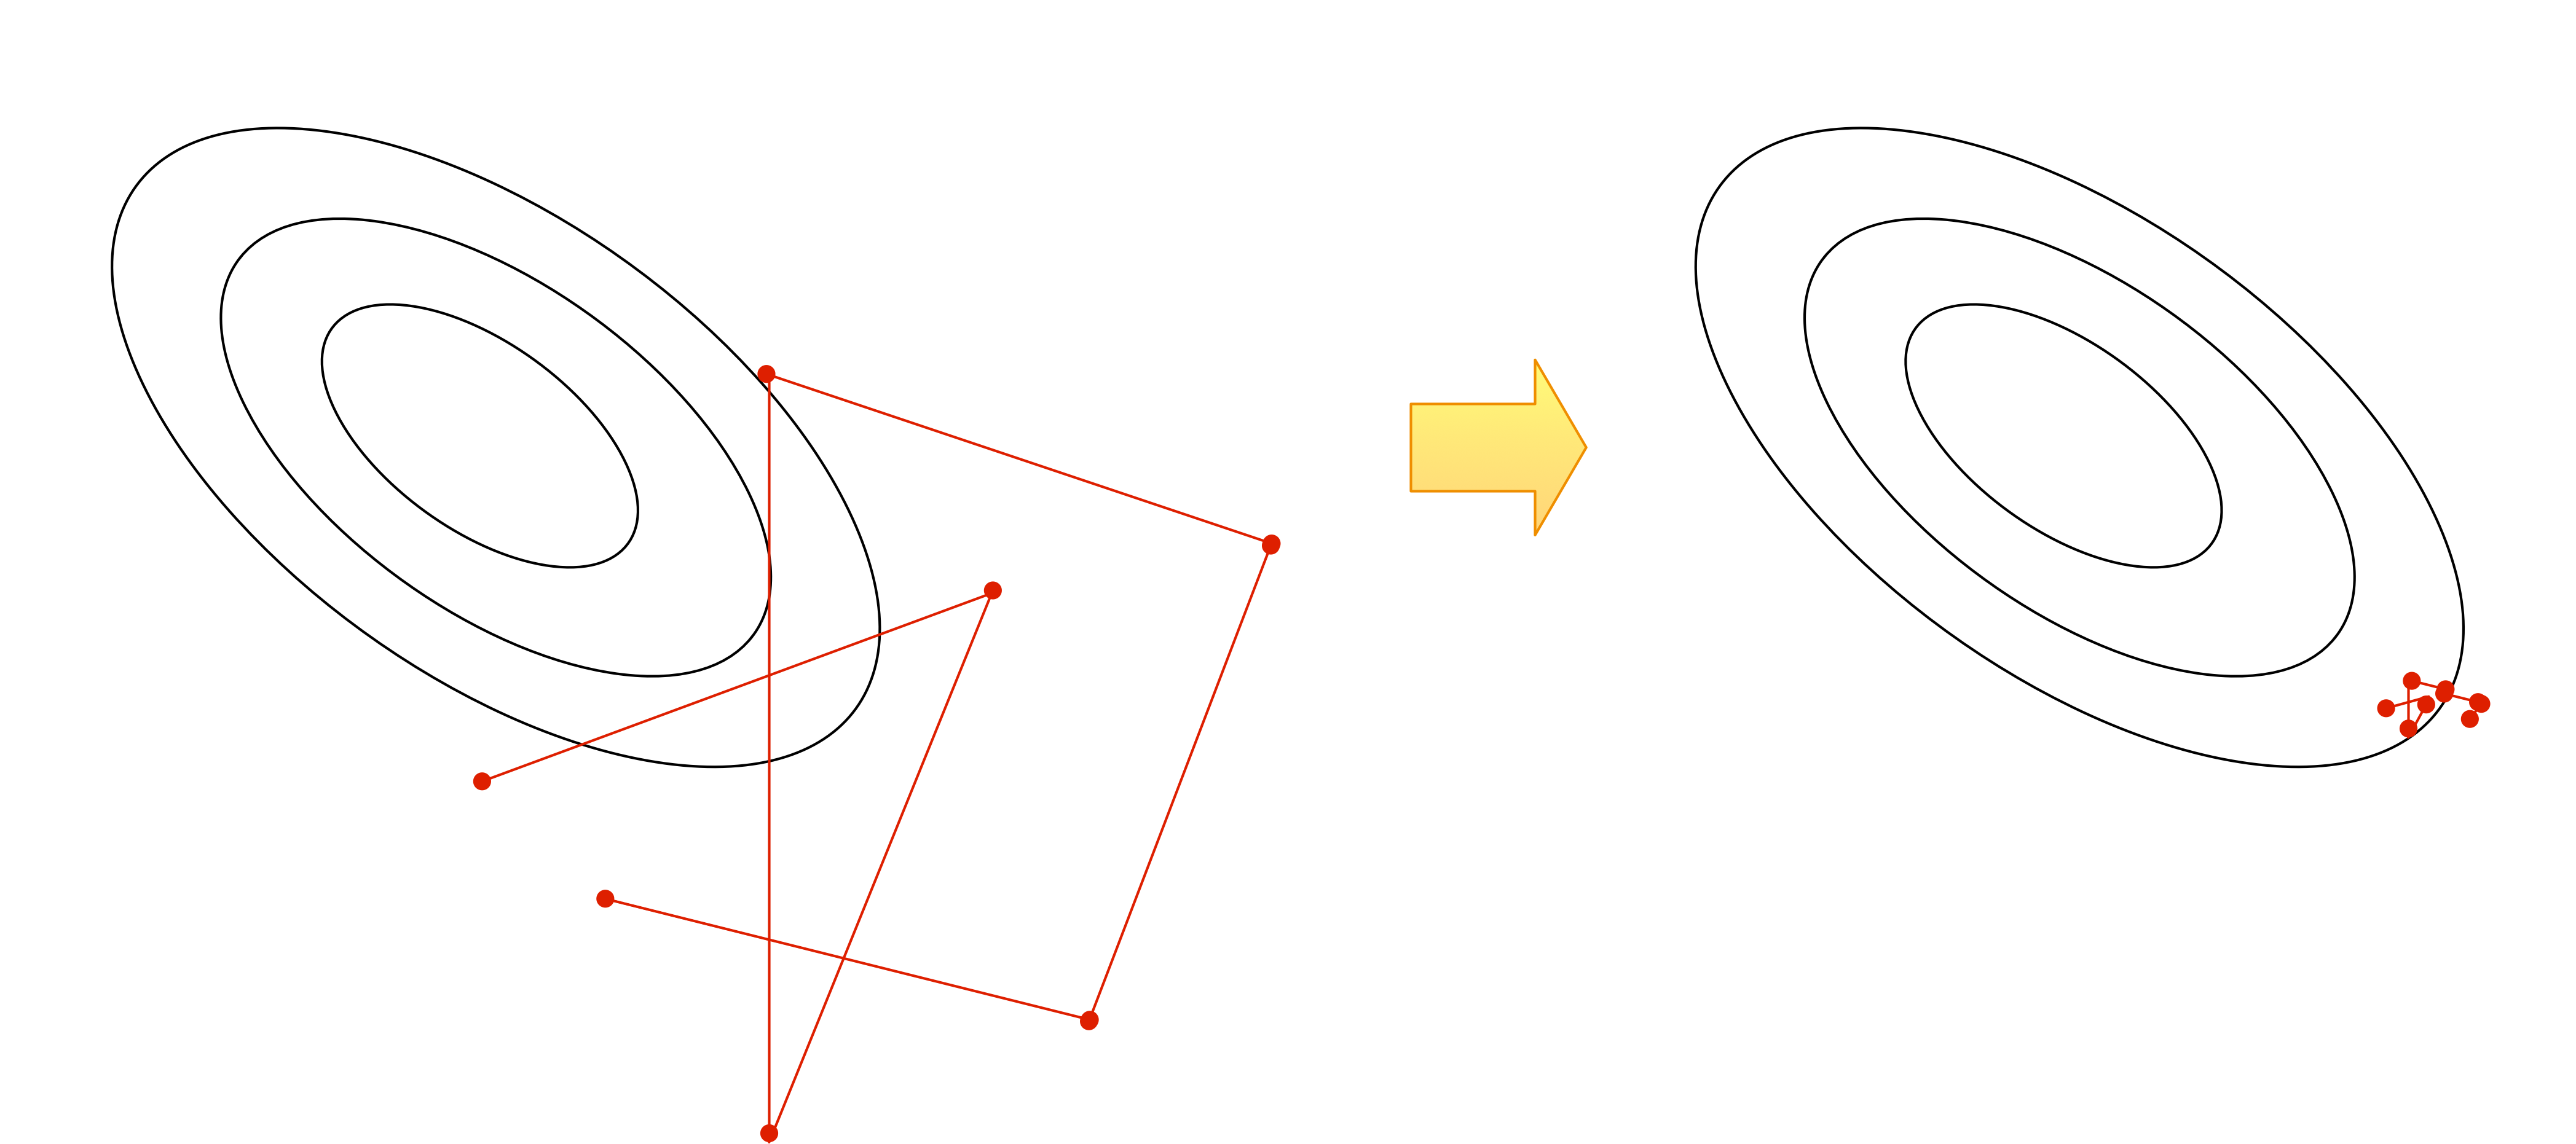
\includegraphics[width=0.25\linewidth]{figures/premature_lr_decay.png}
      \hspace{0.05 \linewidth}
      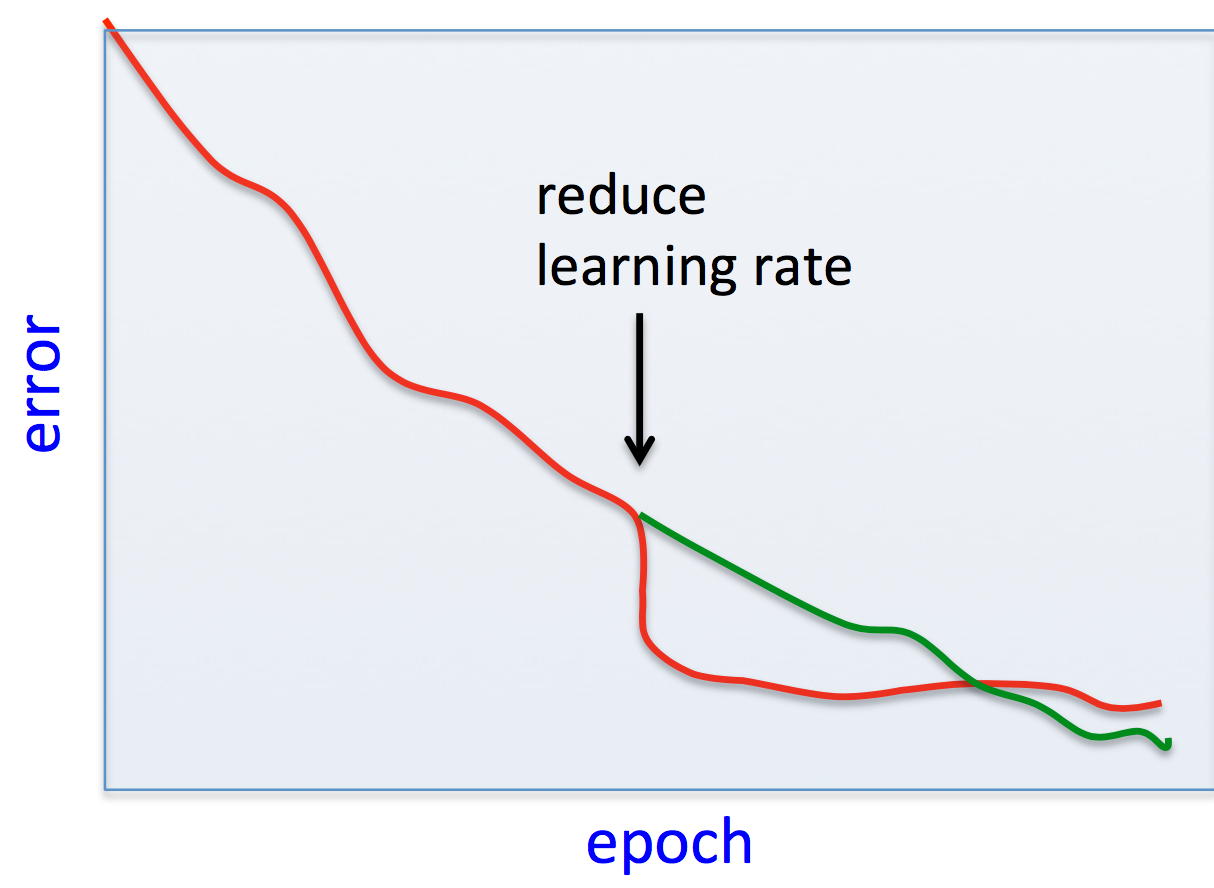
\includegraphics[width=0.25\linewidth]{figures/sgd_learning_curves.png}
    \end{center}
\end{frame}

\begin{frame}{RMSprop and Adam}
  \begin{itemize}
  \item Recall: SGD takes large steps in directions of high curvature and small steps in directions of low curvature.
  \item \alert{RMSprop} is a variant of SGD which rescales each coordinate of the gradient to have norm 1 on average. It does this by keeping an exponential moving average $s_j$ of the squared gradients.
  \item The following update is applied to each coordinate $j$ independently:
    \begin{align*}
      s_j &\gets (1-\gamma) s_j + \gamma [\tfrac{\partial L}{\partial \theta_j}]^2 \\
      \theta_j &\gets \theta_j - \frac{\alpha}{\sqrt{s_j + \epsilon}} \frac{\partial L}{\partial \theta_j}
    \end{align*}
  % \item Both optimizers are included in TensorFlow, Pytorch, etc.
  \end{itemize}
  % \notenew{
  % \begin{itemize}
  %   \item Draw a skewed axis-aligned quadratic.
  %   \item If the eigenvectors of the Hessian are axis-aligned (dubious assumption), then RMSprop can correct for the curvature. In practice, it typically works slightly better than SGD.
  % \end{itemize}
  % }
\end{frame}

\begin{frame}{Adam optimizer}
\begin{columns}
\begin{column}{0.6\textwidth}
\begin{itemize}
  \item \alert{Adam} = RMSprop + momentum = Adaptive Momentum estimation
  \item Smoother estimate of the average gradient and gradient norm.
  \item $m_t$: exponential moving average of gradient.
  \item $v_t$: exponential moving average of gradient squared.
  \item $\hat{m}_t$, $\hat{v}_t$: Bias correction.
  \item $\theta_t \leftarrow \theta_{t-1} - \alpha \hat{m}_t / (\sqrt{\hat{v_t}} + \epsilon)$
  \item The ``default'' optimizer for modern networks.
\end{itemize}
\end{column}
\begin{column}{0.38\textwidth}
\begin{center}
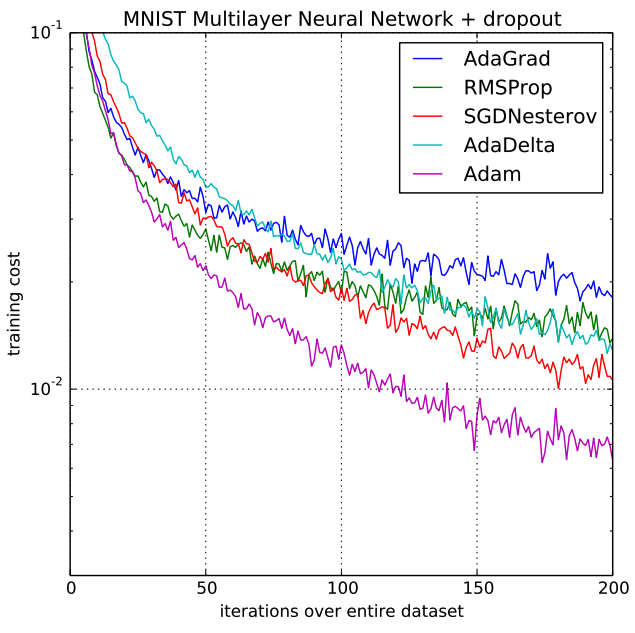
\includegraphics[width=0.8\textwidth]{figures/adam.png}
\end{center}
\end{column}
\end{columns}
\end{frame}

\begin{frame}{Normalization}
% \begin{columns}
% \begin{column}{0.6\textwidth}
\begin{itemize}
    \item Weight initialization is tricky, and there is no guarantee that the distribution of activations will stay the same over the learning process.
    \item What if the weights keep grow bigger and activation may explode?
    \item We can ``normalize'' the activations.
    \item The idea is to control the activation within a normal range: zero-mean, uni-variance.
\end{itemize}
% \end{column}
% \begin{column}{0.38\textwidth}
% \begin{center}
% 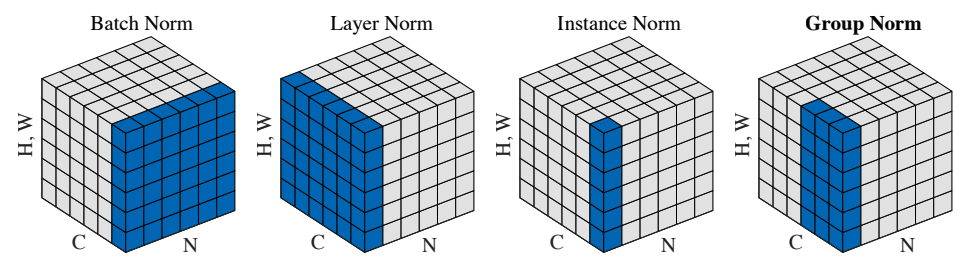
\includegraphics[width=0.8\textwidth]{figures/normalization.png}
% \end{center}
% \end{column}
% \end{columns}
\end{frame}

\begin{frame}{Batch Normalization (BN)}

\begin{columns}
\begin{column}{0.6\textwidth}
\begin{itemize}
    % \item What is the population to normalize it from?
    \item Training image distribution -> activation distribution
    \item In CNNs, neurons across different spatial locations are also samples of the same feature channel.
    \item Batch norm: Normalize across N H W dimensions, leaving C channels.
    \item $\tilde{x} = \gamma \frac{x - \mu}{\sigma} + \beta$
    \item Test time: using the mean and variance from the entire training set.
\end{itemize}
\end{column}

\begin{column}{0.38\textwidth}
\begin{center}
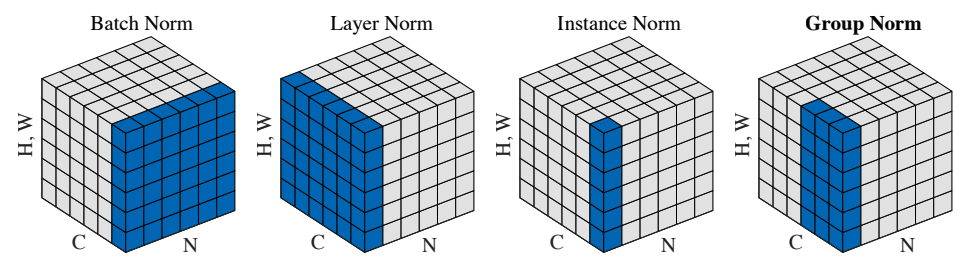
\includegraphics[width=0.7\textwidth,trim={0 0 25.5cm 0},clip]{figures/normalization.png}
\end{center}
\end{column}
\end{columns}

\end{frame}

\begin{frame}{BN Alternatives}
\begin{itemize}
    \item Need a considerable batch size to estimate mean and variance correctly.
    \item Training is different from testing.
    \item Alternatives consider the C channel dimension instead of N batch dimension.
    % \item No longer estimating the distribution from training samples.
\end{itemize}
\begin{center}
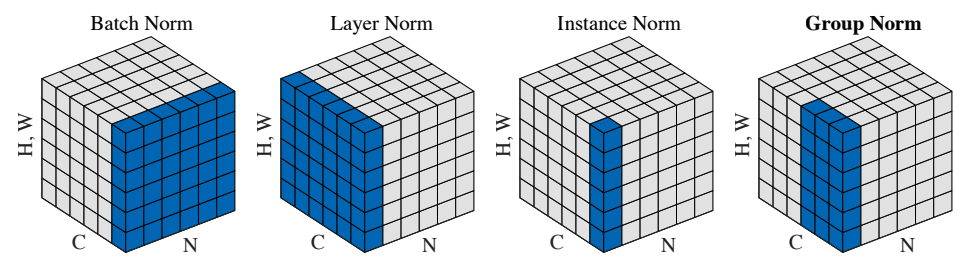
\includegraphics[width=0.7\textwidth,trim={10cm 0 0 0},clip]{figures/normalization.png}
\end{center}
\end{frame}

\begin{frame}{Going Deeper}
\begin{itemize}
    \item The progress of normalization allowed us to train even deeper networks.
    \item The networks are no longer too sensitive with initialization.
    \item But the best networks were still around 20 layers and deeper results in worse performance.
\end{itemize}
\begin{center}
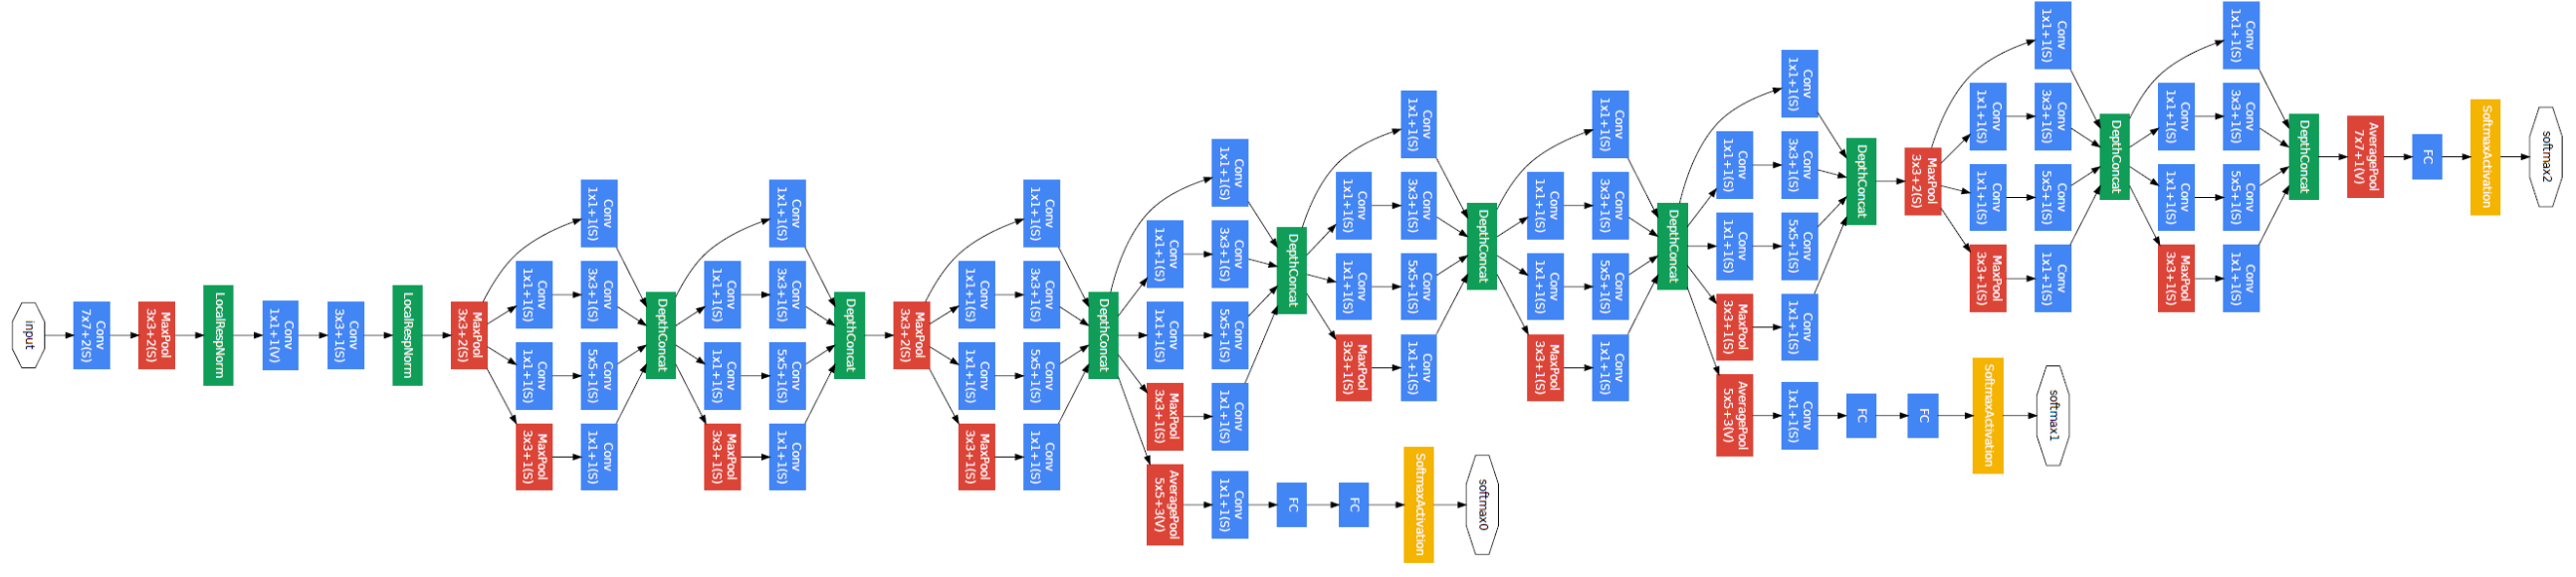
\includegraphics[width=0.6\textwidth]{figures/googlenet.png}
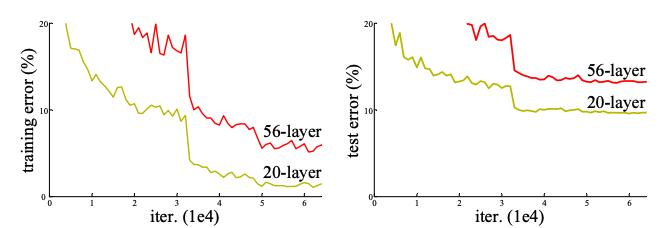
\includegraphics[width=0.35\textwidth]{figures/20layer.png}
\end{center}
\end{frame}

\begin{frame}{Residual Networks (ResNet)}

\begin{itemize}
    \item Recall in gradient boosting, we are iteratively adding a function to the model to expand the capacity.
    \item Residual connection: Skip connection to prevent gradient vanishing.\footnote{He et al. Deep Residual Learning for Image Recognition. CVPR 2016.}
    % \item A simple ``addition'' operation on the activation.
\end{itemize}

\begin{center}
% 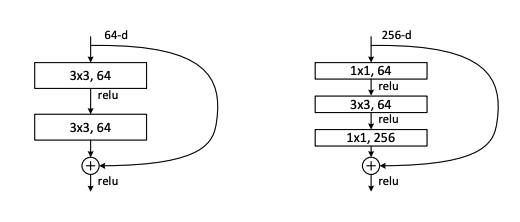
\includegraphics[width=0.75\textwidth]{figures/residual_connect.png}
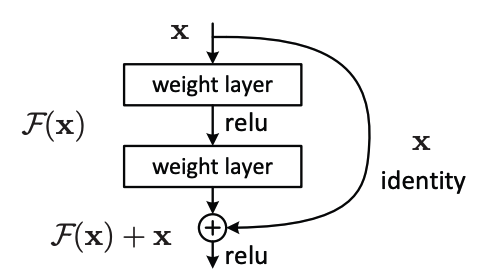
\includegraphics[width=0.5\textwidth]{figures/resnet.png}
\end{center}

\end{frame}

\begin{frame}{ResNet Success}
\begin{itemize}
    \item Now able to train over 100 layers.
    \item One of the most important network design choices in the past decade.
    \item Prevalent in almost all network architectures, including Transformers.
    \item Loss landscape view: Skip connections makes loss smoother -> easier to optimize \footnote{Li et al. Visualizing the Loss Landscape of Neural Nets. NIPS 2018.}.
\end{itemize}
\begin{center}
% 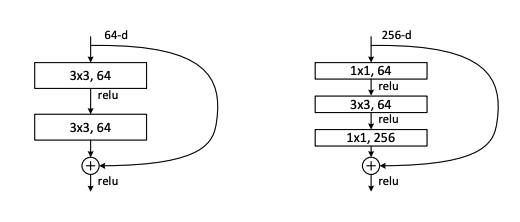
\includegraphics[width=0.75\textwidth]{figures/residual_connect.png}
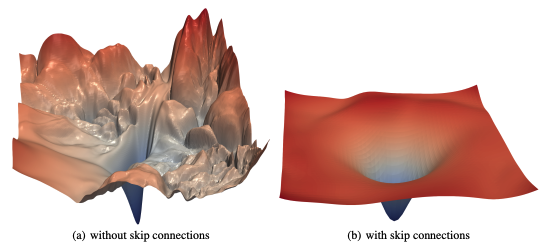
\includegraphics[width=0.5\textwidth]{figures/resnetlandscape.png}
\end{center}
\end{frame}

\begin{frame}{Dropout\footnote{Srivastava et al. A Simple Way to Prevent Neural Networks from Overfitting. JMLR, 2014.}
}
\begin{itemize}
    \item Want to reduce overfitting in neural networks.
    \item Stochastically turning off neurons in propagation.
    \onslide<2->{
    \item Training to preserve redundancy.
    \item Test time: multiplying activations with probability. Model ensembling effect.
    }
\end{itemize}
\begin{center}
\onslide<1->{
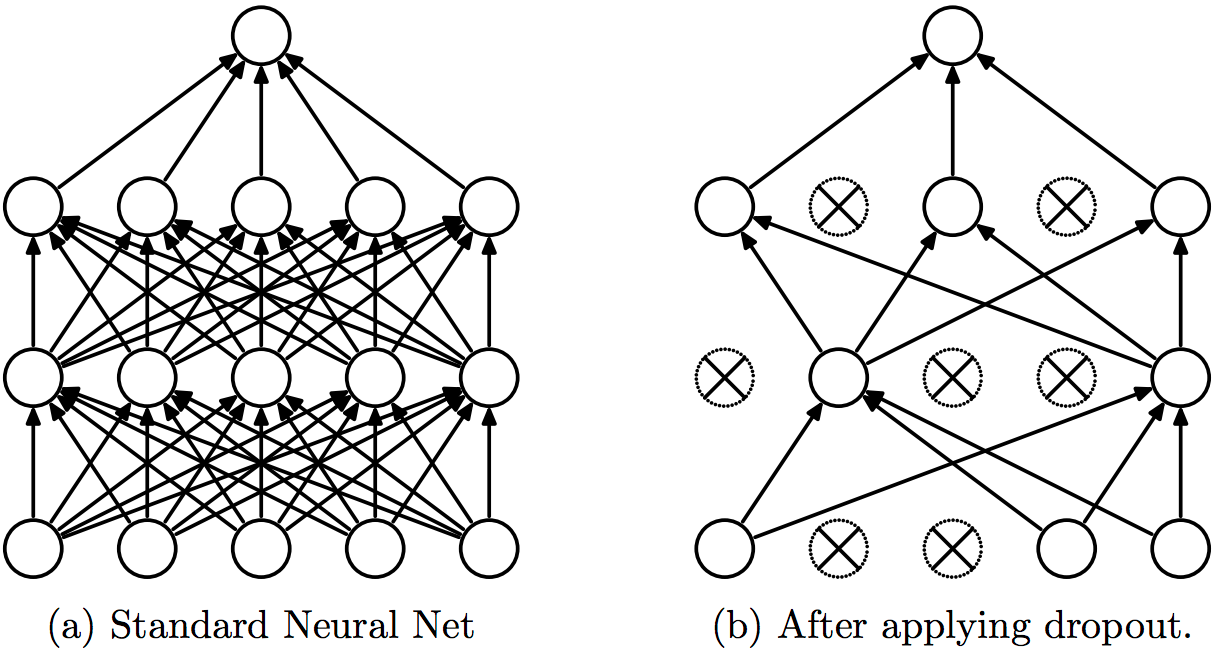
\includegraphics[width=0.4\textwidth]{figures/dropout.png}
}
\end{center}

\end{frame}

\begin{frame}{GELU\footnote{Hendrycks \& Gimpel. Gaussian Error Linear Unit (GELU). CoRR abs/1606.08415, 2016.}}
\begin{columns}
\begin{column}{0.49\textwidth}
\begin{itemize}
    \item Gaussian Error Linear Unit - A smoother activation function. 
    \item Motivated by Dropout.
    \onslide<2->{
    \item $f(x) = \mathbb{E}[x \cdot m].$
    }
    \onslide<3->{
    \item $m \sim Bernoulli(\Phi(x)).$
    \item $\Phi(x) = P(X \le x).$
    \item $X \sim \mathcal{N}(0,1).$
    }
\end{itemize}
\end{column}
\begin{column}{0.49\textwidth}
\begin{center}
    \onslide<1->{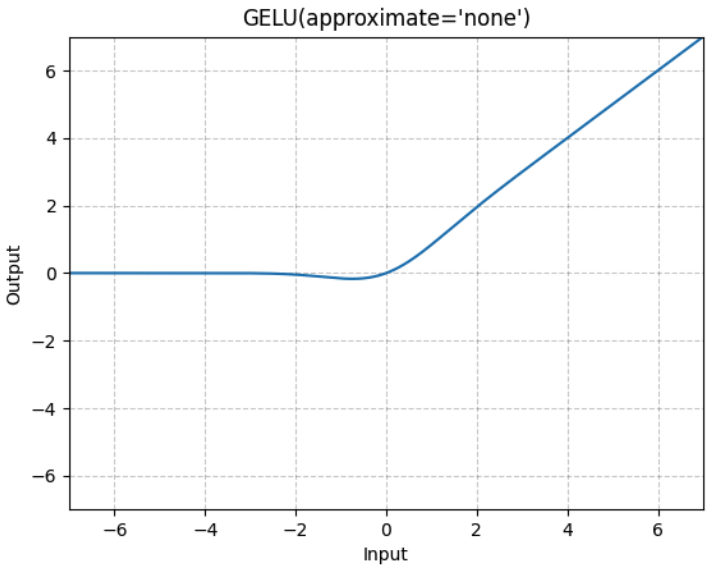
\includegraphics[width=0.8\textwidth]{figures/gelu.png}}
\end{center}
\end{column}
\end{columns}
\end{frame}

\begin{frame}{Data augmentation}
\begin{columns}
\begin{column}{0.4\textwidth}
\begin{itemize}
    \item Leverage the invariances of images
    \item Create more data points for free
    \begin{itemize}
    \item<2->Random cropping
    \item<3->Left+right flipping
    \item<4->Random color jittering
    \item<5->Random blurring
    \item<6->Affine warping
    \item<6->Etc.
    \end{itemize}
\end{itemize}
\end{column}
\begin{column}{0.59\textwidth}
\onslide<1->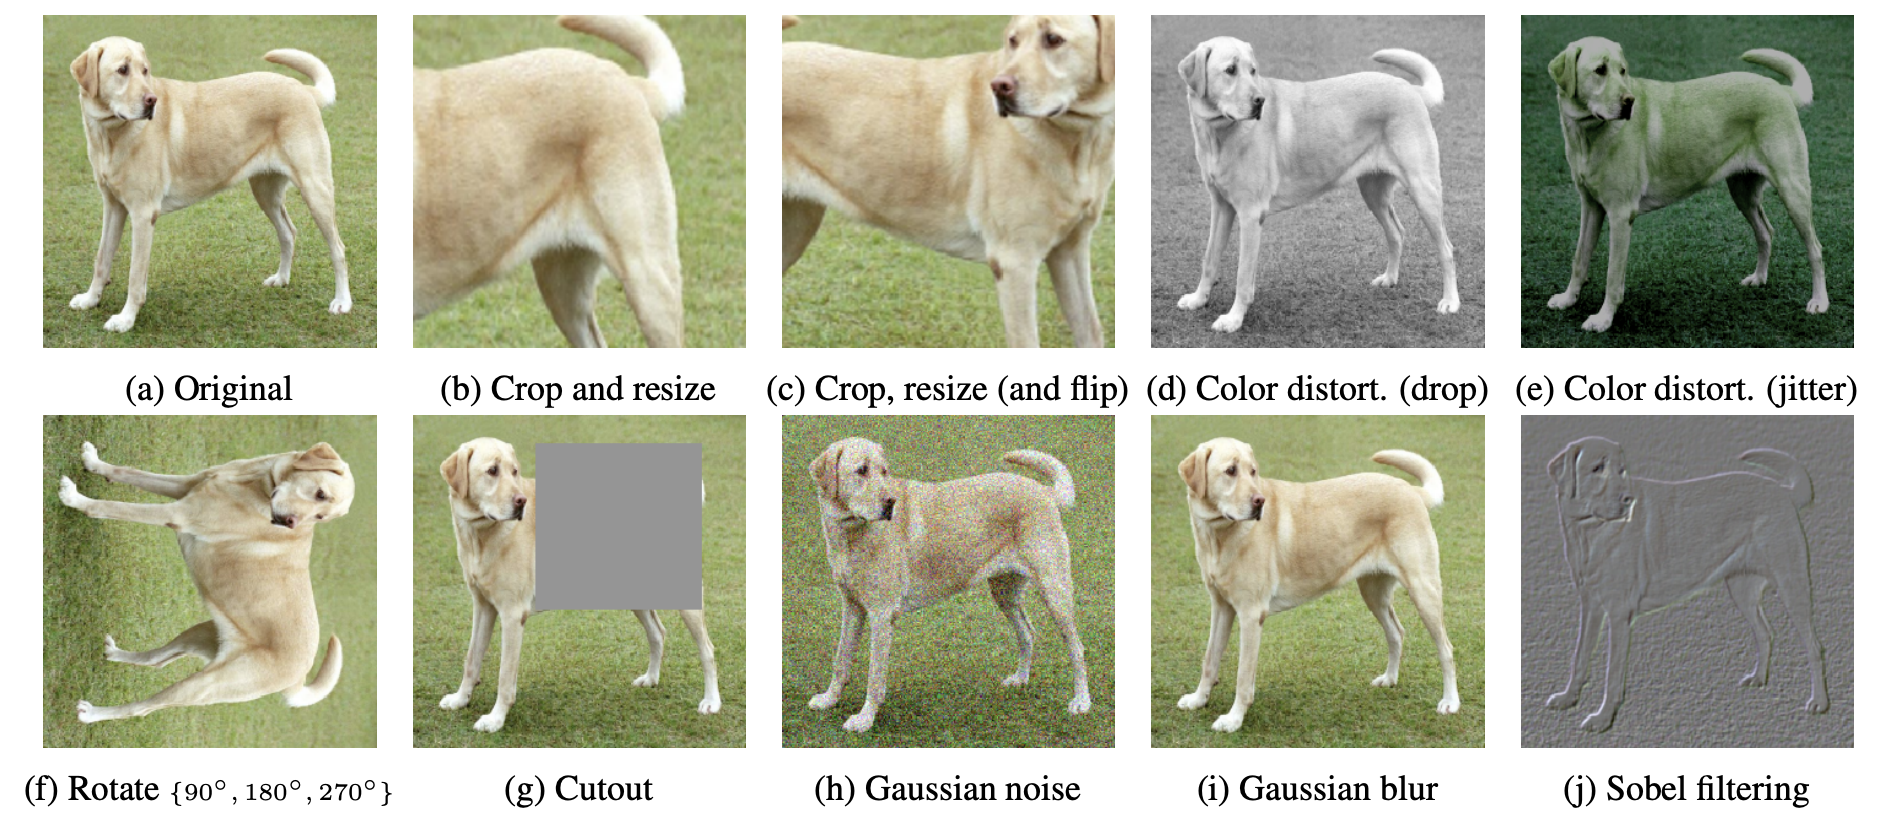
\includegraphics[width=0.9\textwidth]{figures/data_aug.png}
\end{column}
\end{columns}
    \small{Image credit}\footnote{Chen et al. A Simple Framework for Contrastive Learning of Visual Representations. ICML 2020.}
\end{frame}

\section{Language and sequential signals}
\begin{frame}{What about natural language}
\begin{itemize}
    \item<+-> Neural networks are great for dealing with naturalistic and unstructured signals.
     % such as images, sound, language, where there are no good manual feature extractors.
    \item<+-> Past lectures: Feature functions in structured models, but still primitive.
    \item<+-> Design neural networks to accomodate sequential signals such as language.
\end{itemize}
\begin{center}
\onslide<1->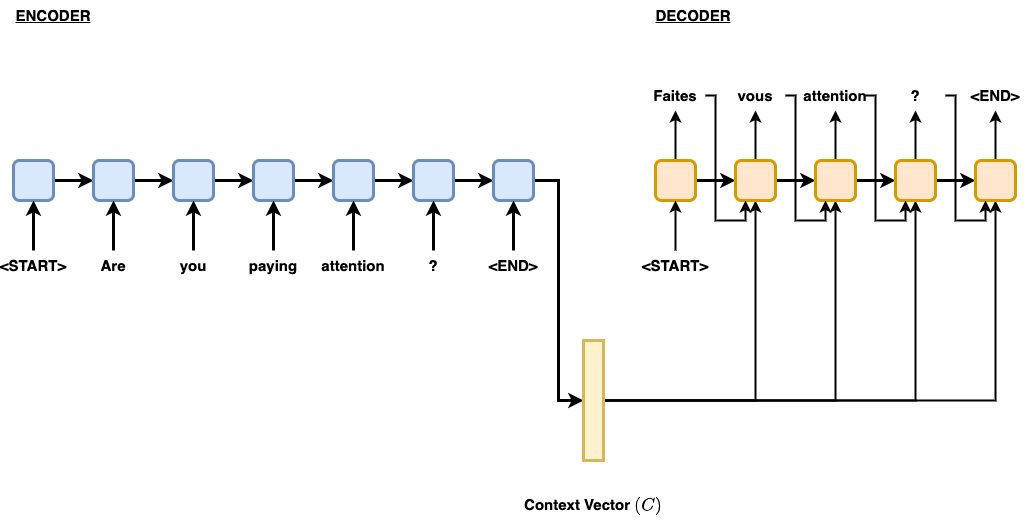
\includegraphics[width=0.7\textwidth,trim={0 0 0 3cm},clip]{figures/neural-machine-translation.png}
\end{center}
\end{frame}

\begin{frame}{Word embeddings}
\begin{itemize}
    \item<+-> Neural networks are best dealing with real valued vectors.
    \item<+-> Need to convert words (discrete) into vectors (continuous).
    \item<+-> A large matrix of $V \times D$. V = vocab size, D = network embedding size.
\end{itemize}
\begin{center}
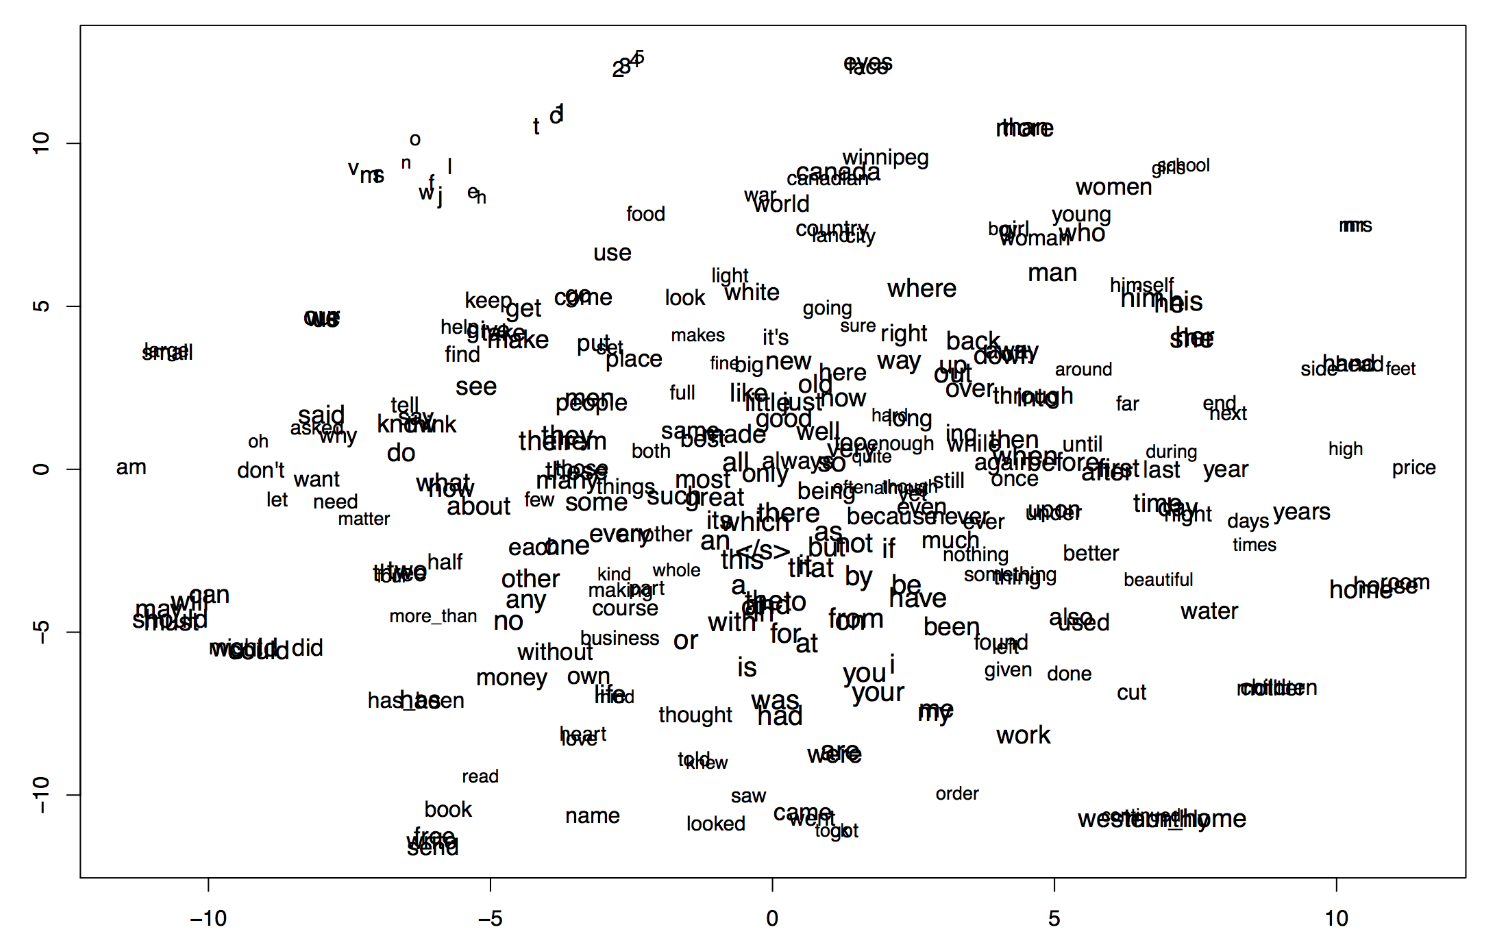
\includegraphics[width=0.4\textwidth]{figures/word_embedding.png}\footnote{https://aelang.github.io/word-embeddings.html}
\end{center}
\end{frame}

\begin{frame}{Convolutional vs. recurrent networks}
\begin{itemize}
    \item Recall in images we used the convolution operation.
    \item We can also use the idea of convolution for temporal signals.
    \item Another alternative is to use a type of network called recurrent networks.
    \item Two inputs: $\mathbf{x}_t$ is the current input, and $\mathbf{h}_t$ is the historical hidden state.
    \item We can unroll the computation graph into a direct acyclic graph (DAG).
\end{itemize}
\begin{center}
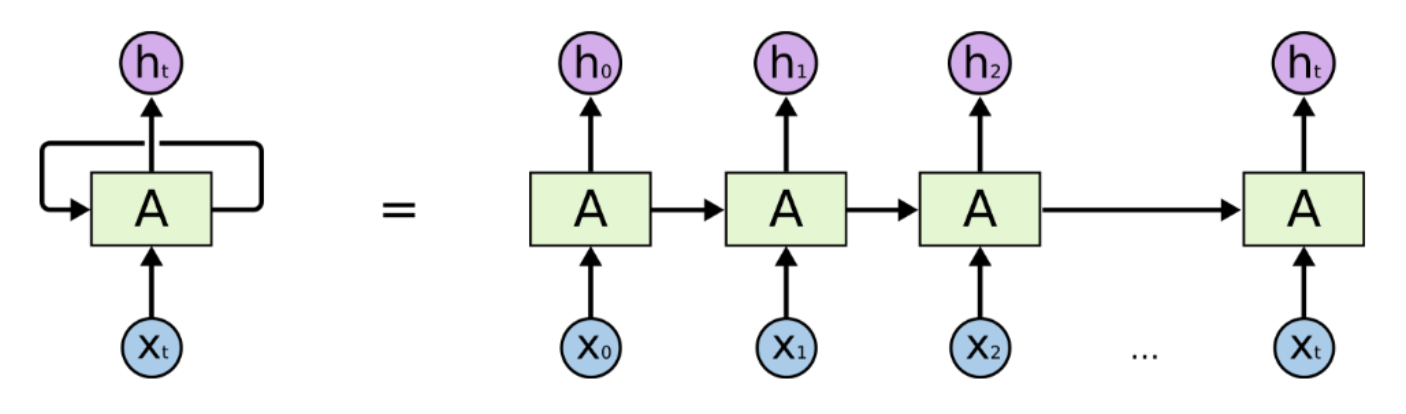
\includegraphics[width=0.7\textwidth]{figures/rnn.png}
\end{center}
\end{frame}

\begin{frame}{Recurrent neural networks (RNNs)}
\begin{itemize}
  \item<+-> A simple RNN can be made similar to a standard NN with one hidden layer.
  \item $h_{t} = \tanh(W h_{t-1} + U x_{t})$.
  \item $y_{t} = \softmax(V h_t)$.
\end{itemize}
\begin{center}
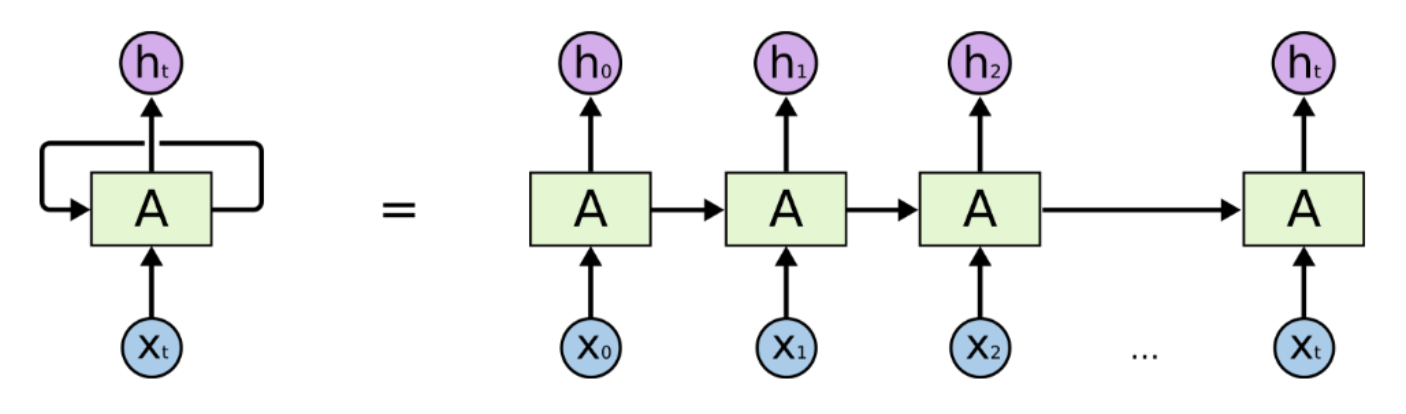
\includegraphics[width=0.7\textwidth]{figures/rnn.png}
\end{center}
\footnote{Image credit: Chris Olah~\url{https://colah.github.io/posts/2015-08-Understanding-LSTMs/}}
\end{frame}

\begin{frame}{Gradient vanishing}
\begin{itemize}
  \item<+-> Every iteration, we multiply the hidden state $h_{t-1}$ from the previous iteration with the same $W$.
  \item<+-> If the largest singular value of $W$ is less than one then back-propagation will be attenuated.
  \item<+-> Similarly, we apply $\tanh$ activation every iteration -- further reducing gradient flow.
\end{itemize}
\begin{center}
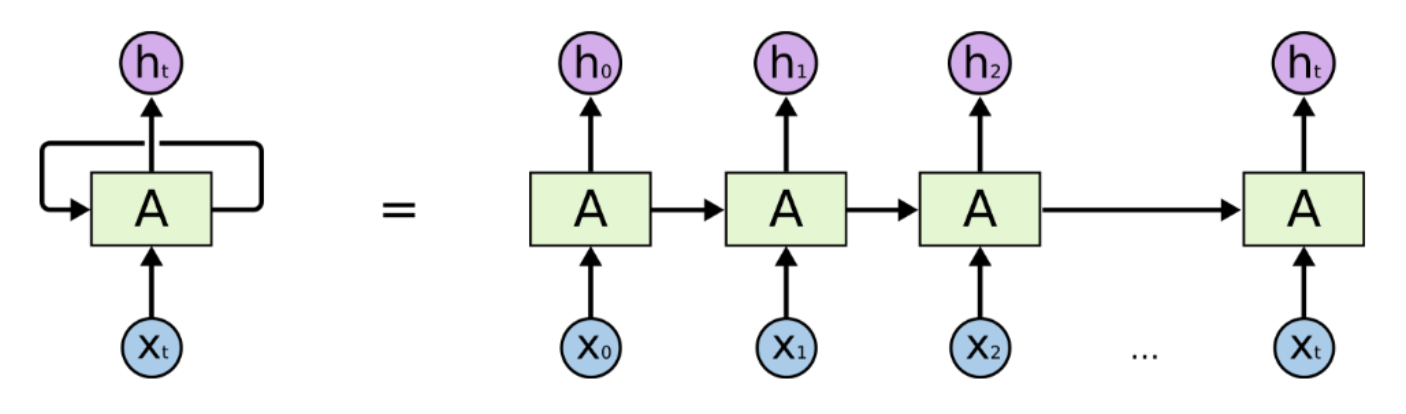
\includegraphics[width=0.7\textwidth]{figures/rnn.png}
\end{center}
\end{frame}

\begin{frame}{Gating functions in LSTM}
\begin{itemize}
    \item Long short-term memory is a network that addresses the gradient vanishing problem by introducing gating functions.
    \item Gating functions provide ``shortcuts'', like ResNet.
    \item Originally proposed by Hochreiter and Schmidhuber in 1997.
\end{itemize}
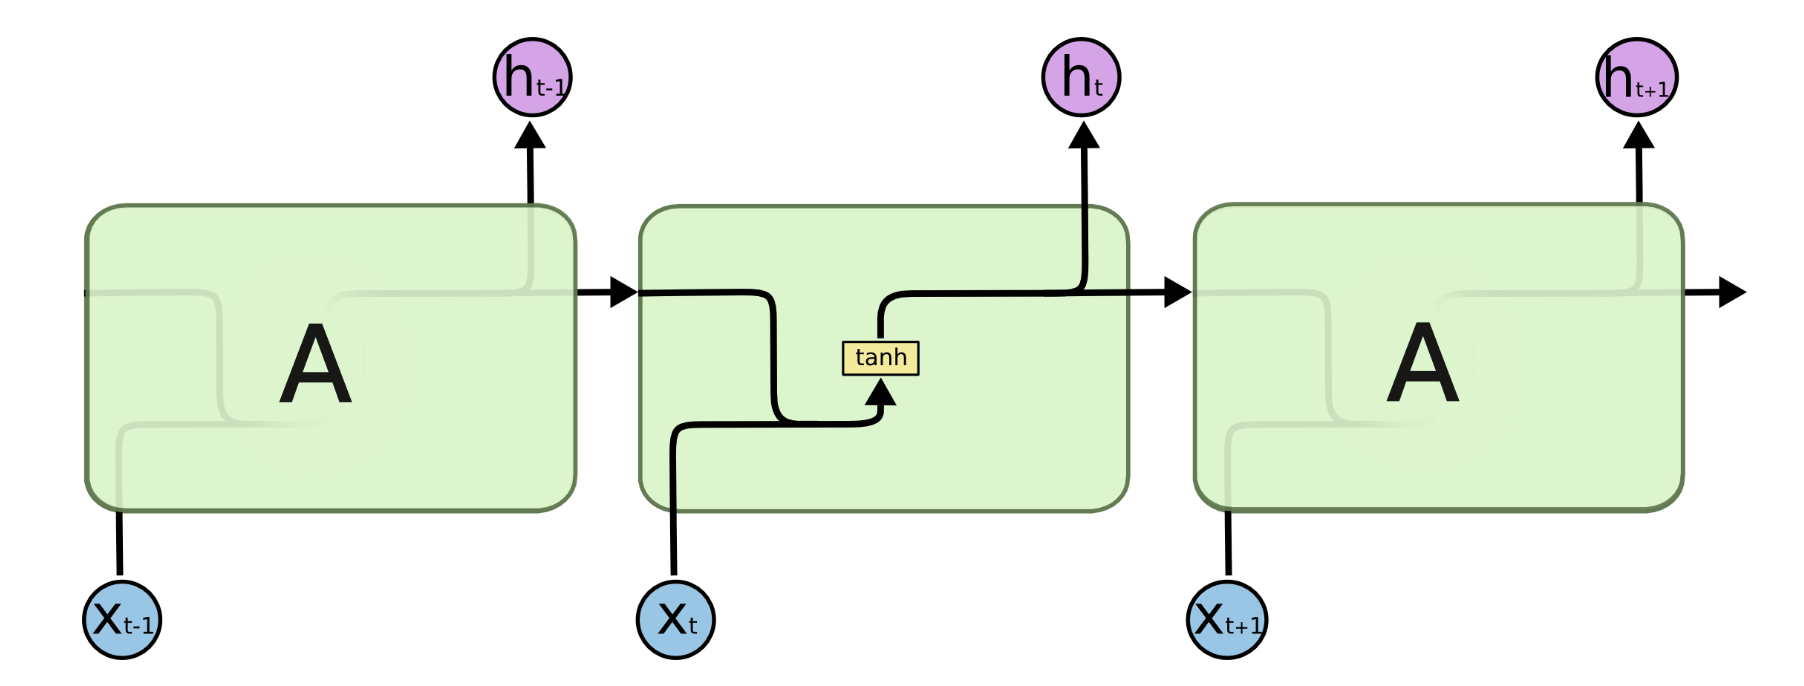
\includegraphics[width=0.49\textwidth]{figures/rnn_cell.png}
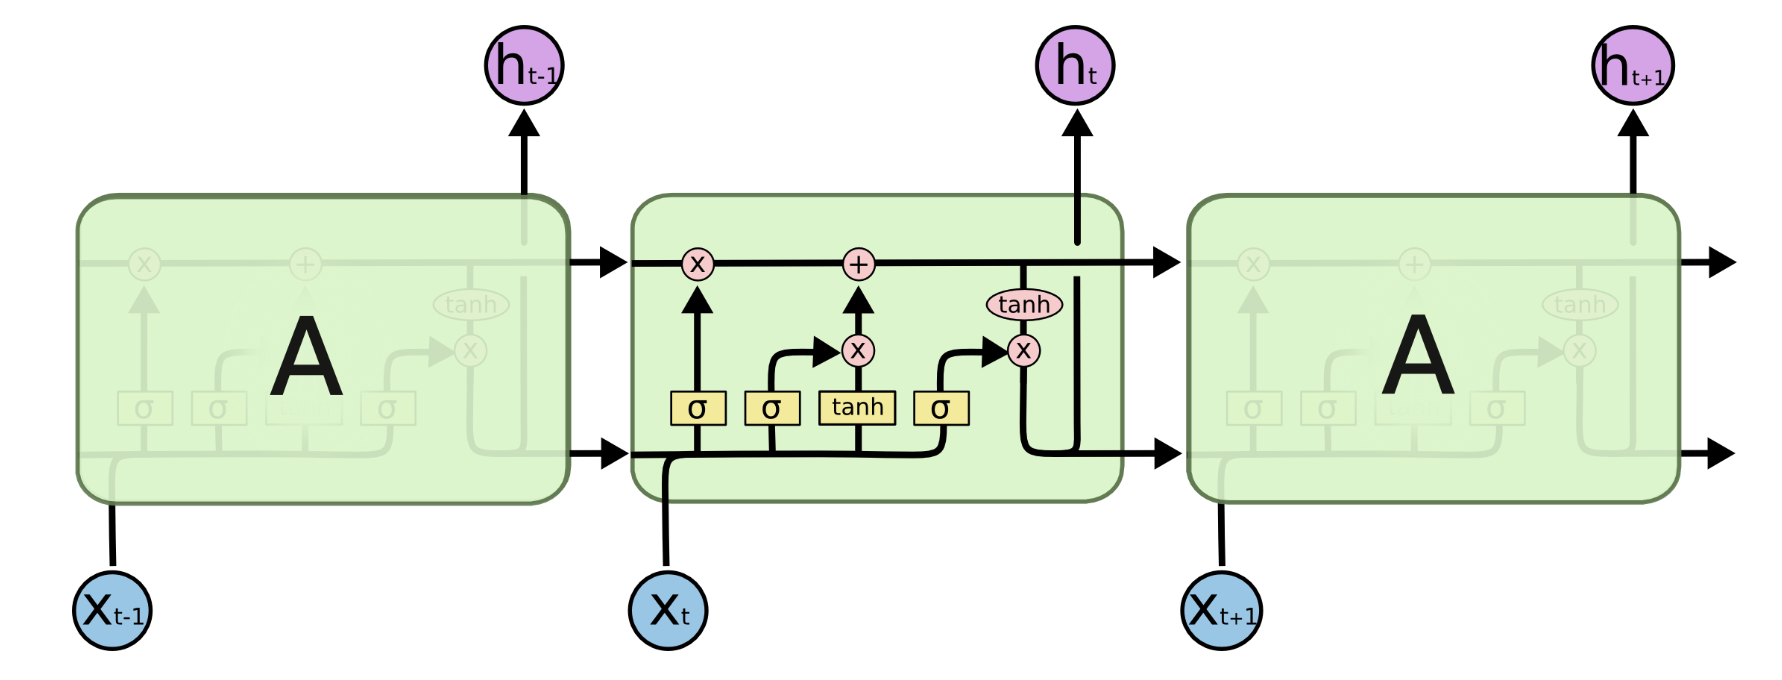
\includegraphics[width=0.49\textwidth]{figures/lstm_cell.png}
\end{frame}

\begin{frame}{Gating functions in LSTM}
\begin{columns}
\begin{column}{0.5\textwidth}
\begin{itemize}
    \item<+-> Input gate: $i_t = \sigma(W_i [h_{t-1}, x_t] + b_i)$.
    \item<1-> Forget gate: $f_t = \sigma(W_f [h_{t-1}, x_t] + b_f)$.
    \item<1-> $z_t = \tanh(w_z [h_{t-1} x_t] + b_z)$.
    \item<+-> $c_t = f_t \odot c_{t-1} + i_t \odot z_t$.
    \item<+-> Output gate: $\sigma(W_o [h_{t-1}, x_t] + b_o)$.
    \item<3-> $h_t = o_t \odot \tanh(c_t)$.
\end{itemize}
\end{column}
\begin{column}{0.5\textwidth}
\begin{center}
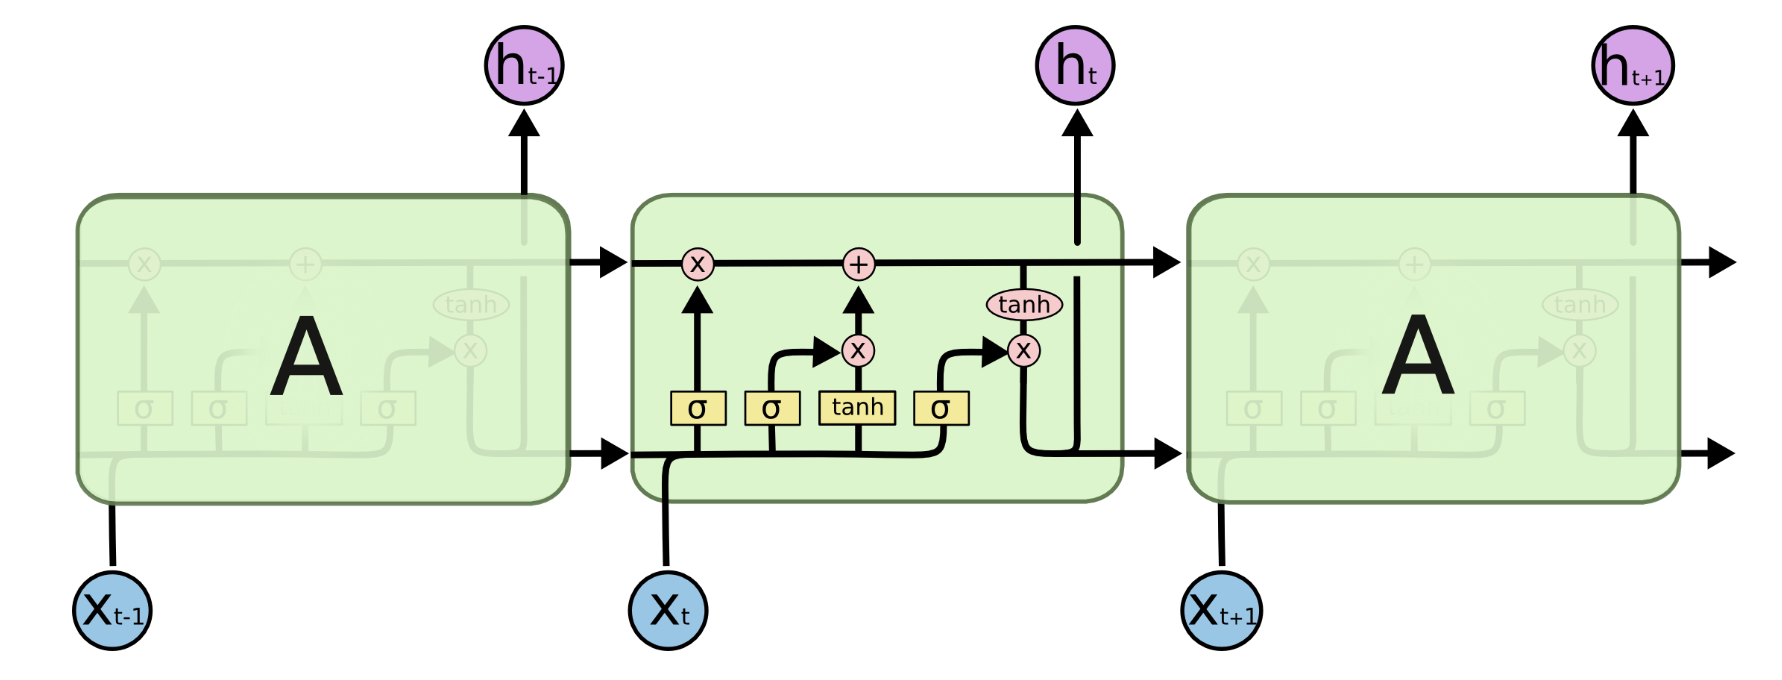
\includegraphics[width=\textwidth]{figures/lstm_cell.png}
\end{center}
\end{column}
\end{columns}
\end{frame}

\begin{frame}{Gated Recurrent Unit}
\begin{columns}
\begin{column}{0.5\textwidth}
\begin{itemize}
    \item<+-> Proposed by Chung et al. in 2015, a simplified variant compared to LSTM.
    \item<+-> Input gate $i_t = \sigma(W_i [h_{t-1}, x_t] + b_i)$.
    \item<+-> Reset gate $r_t = \sigma(W_r [h_{t-1}, x_t] + b_r)$.
    \item<+-> $\tilde{h}_t = \tanh(W_h [r_t \odot h_t, x_t] + b_h)$.
    \item<+-> $h_t = (1-i_t) \odot h_{t-1} + i_t \odot \tilde{h}_t$.
\end{itemize}
\end{column}
\begin{column}{0.5\textwidth}
\begin{center}
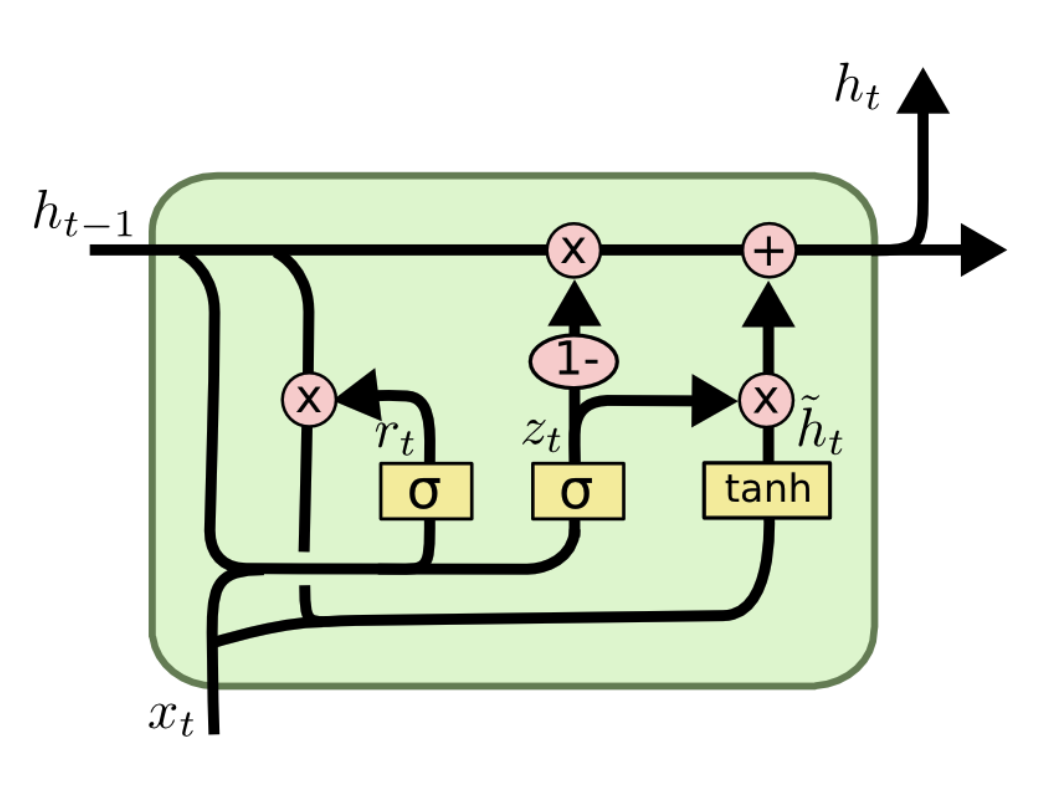
\includegraphics[width=\textwidth]{figures/gru_cell.png}
\end{center}
\end{column}
\end{columns}
\end{frame}

\begin{frame}{Attention Mechanisms}
\begin{columns}
\begin{column}{0.5\textwidth}
\begin{itemize}
    \item Earlier content will decay more.
    \item Hard to refer back to the raw content.
    \item Reverse order better than forward order [abcde -> a'b'c'd'e' vs. abcde -> e'd'c'b'a'].
    \item Attending to arbitrary sequence tokens.
    \item $s_t = f(s_{t-1}, y_{t-1}, c_t)$
    \item $c_t = \sum_\tau \alpha_{t, \tau} h_\tau$, $\alpha_{t,\tau} = \frac{\exp(a_(s_{t-1},h_k))}{\sum_{k} \exp(a_(s_{t-1},h_k))}$
    \item $a(s_{t-1}, h_k) = v_a^\top \tanh(W_a [s_{i-1}, h_k])$
\end{itemize}
\end{column}
\begin{column}{0.5\textwidth}
\begin{center}
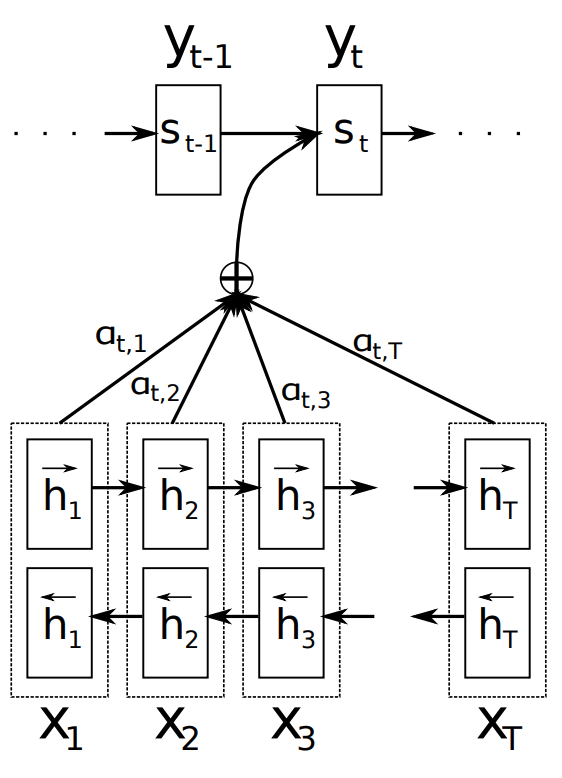
\includegraphics[width=0.6\textwidth]{figures/attention_nmt.png}\\
Bahdanau et al., 2014
\end{center}
\end{column}
\end{columns}
\end{frame}

\begin{frame}{Transformers (``Attention is All You Need'')}
\begin{itemize}
    \item The previous architecture is very complicated.
    {\small
    \begin{itemize}
    \item 1 RNN for encoding the tokens.
    \item Attention mechanisms for accessing content
    \item 1 RNN for combining attended tokens.
    \end{itemize}
    }
    \item RNNs have the ability to incorporate past information, so does attention.
    % \item Just attention is sufficient.
\end{itemize}
\begin{center}
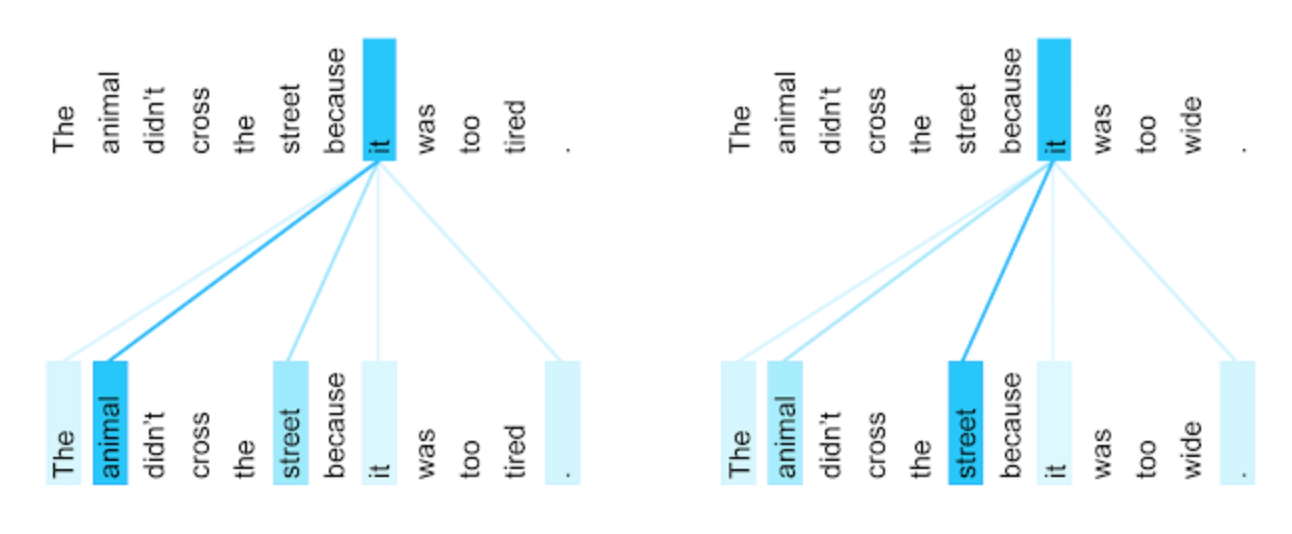
\includegraphics[width=0.4\textwidth]{figures/transformer_attention.png}\\
\footnote{Image credit: \href{https://blog.research.google/2017/08/transformer-novel-neural-network.html}{Google Research Blog}}
\end{center}
\end{frame}

\begin{frame}{Positional encoding}
\begin{itemize}
  \item Attention operation is permuation equivariant.
  % \item We need to encode the sequence order information in the inputs.
  \item Solution: Encode the position of each token.
  \item $PE(pos, 2i) = \sin(p/k^{2i/d}), PE(pos, 2i+1) = \cos(p/k^{2i/d})$.
\end{itemize}
\begin{center}
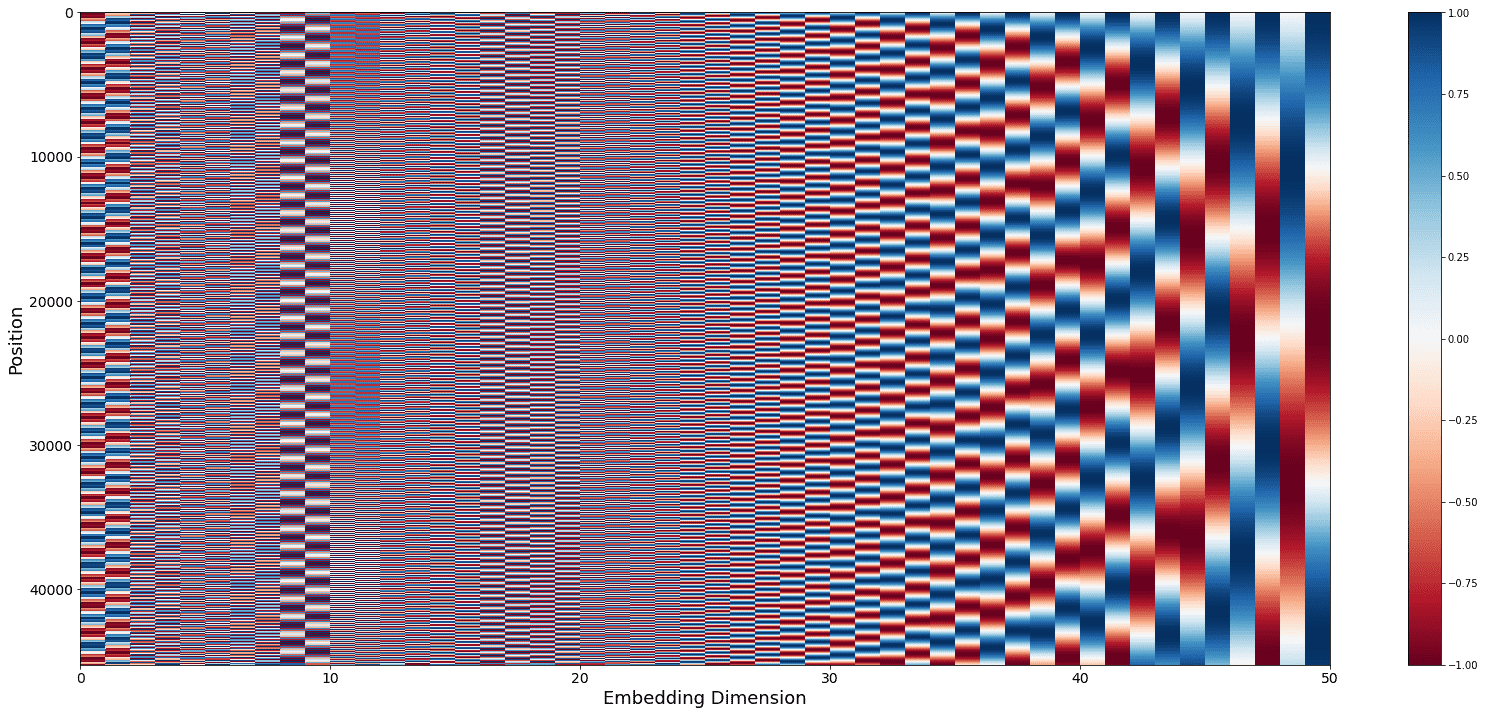
\includegraphics[width=0.6\textwidth]{figures/position_encoding.png}
\end{center}
\end{frame}

\begin{frame}{Multi-headed attention}
\begin{columns}
\begin{column}{0.5\textwidth}
\begin{itemize}
    \item<+-> Map tokens into query, key, and value.
    \item<+-> $Attention(Q,K,V)=\softmax(\frac{Q K^\top}{\sqrt{d_k}})V$.
    \item<+-> $H_i = Attention(Q W_i^Q, K W_i^K, V W_i^V)$.
    \item<+-> $MultiHead(Q, K, V) = [H_1, ..., H_n] W^O$
    % \item<+-> The vanilla form of attention in Bahdanau et al. only considers a single set of softmax values.
    \item<+-> More advantageous to have multiple set of attentions for each token, so it can more efficiently incorporate information from multiple sources.
\end{itemize}
\end{column}
\begin{column}{0.5\textwidth}
\begin{center}
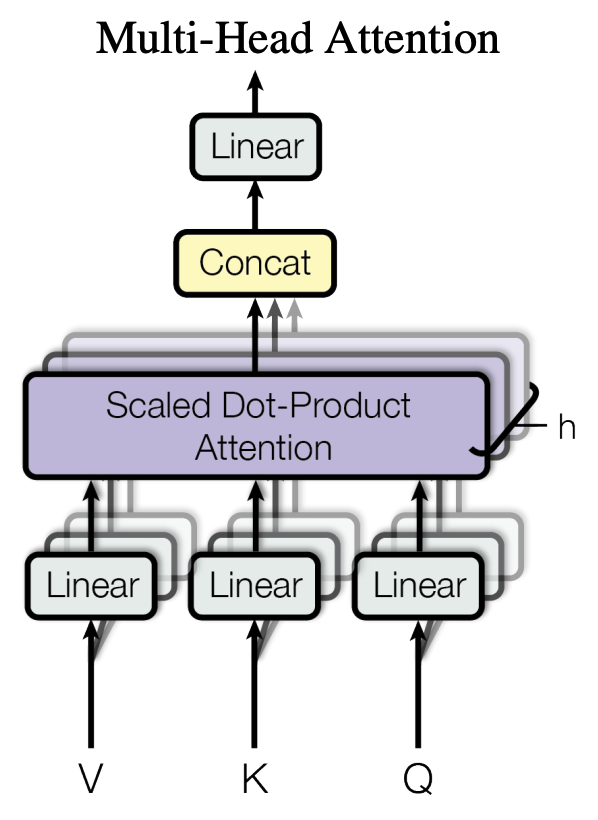
\includegraphics[width=0.5\textwidth]{figures/multi_headed_attention.png}
\end{center}
\end{column}
\end{columns}
\end{frame}

\begin{frame}{Machine Translation}
\begin{itemize}
  \item Achieved superior performance on machine translation.
  \item Animation \href{https://3.bp.blogspot.com/-aZ3zvPiCoXM/WaiKQO7KRnI/AAAAAAAAB_8/7a1CYjp40nUg4lKpW7covGZJQAySxlg8QCLcBGAs/s1600/transform20fps.gif}{link}
\end{itemize}
\begin{center}
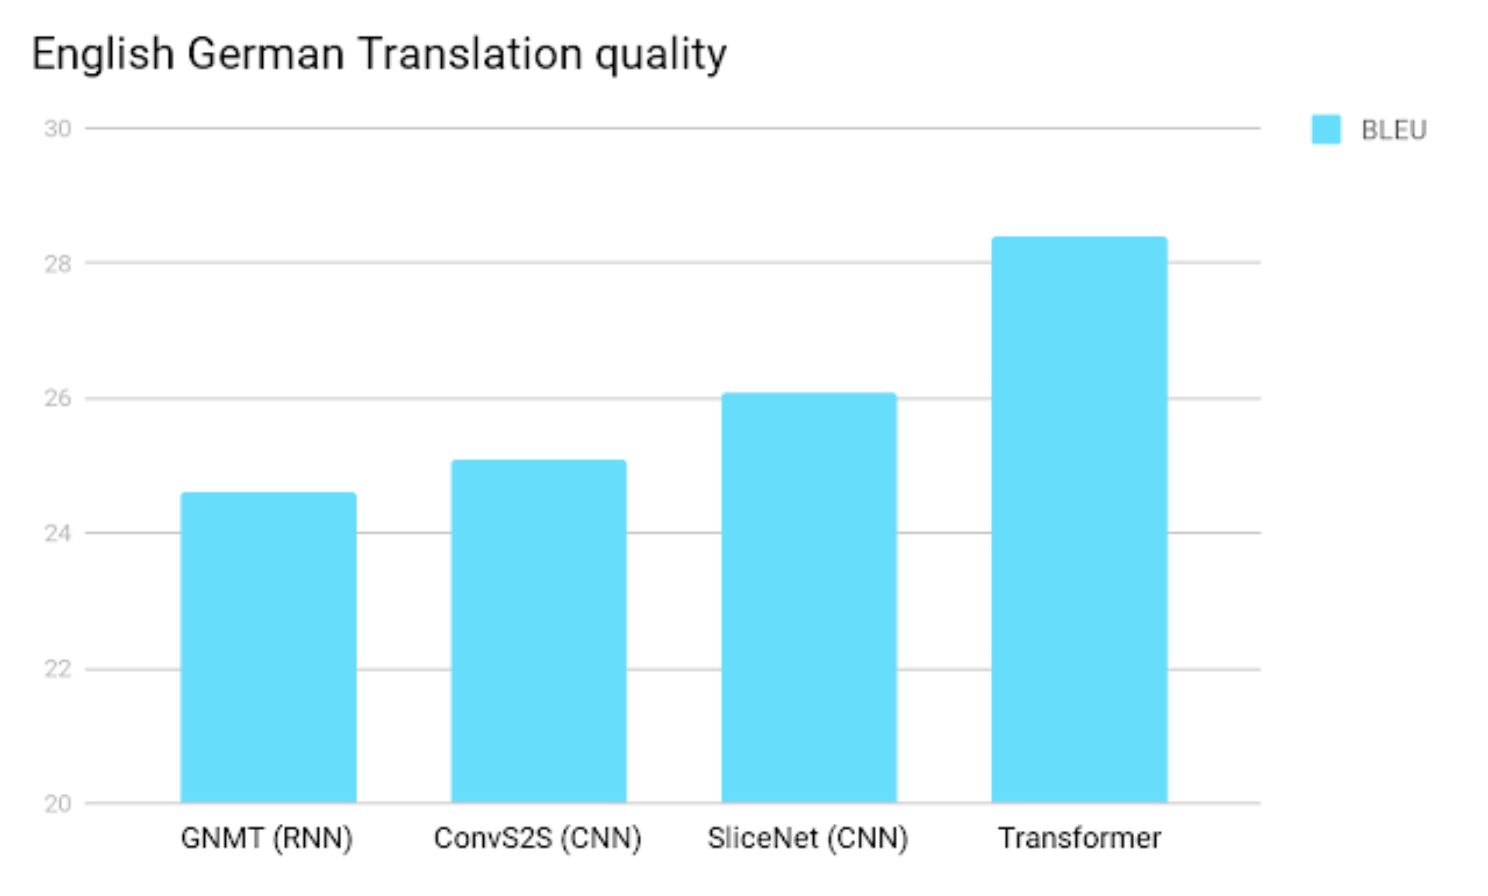
\includegraphics[height=4cm]{figures/en_de.png}
\quad
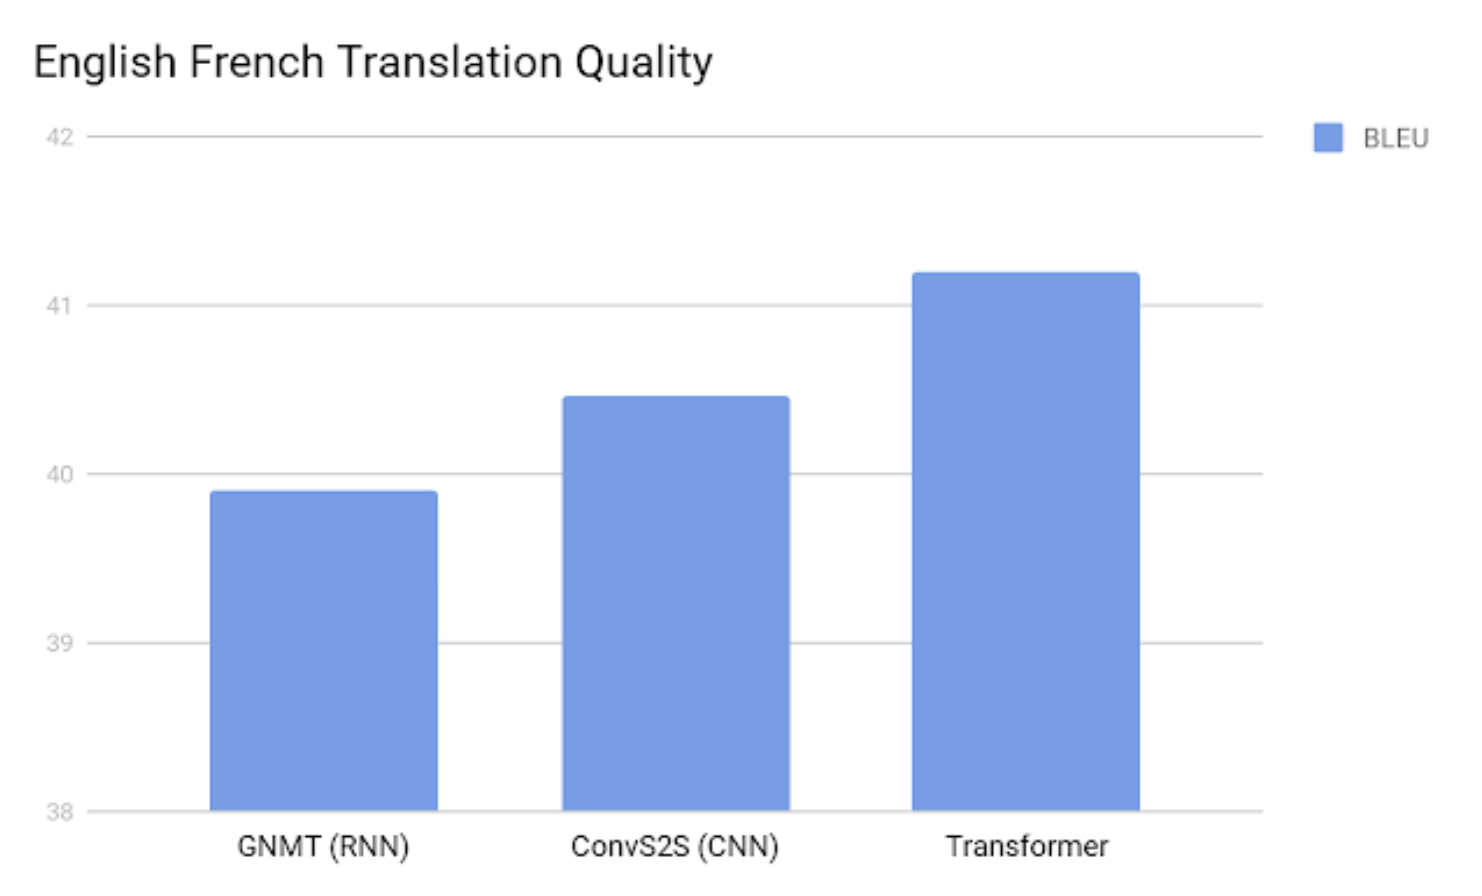
\includegraphics[height=4cm]{figures/en_fr.png}
\end{center}
\end{frame}

\begin{frame}{Autoregressive modeling}
\begin{itemize}
    \item Recall the chain rule on joint distribution:
    \[
    p(x_{1:t}) = p(x_1, \dots, x_t) = p(x_1) p(x_2 | x_1) \dots p(x_t | x_{t-1}) = p(x_1) \prod_i p(x_i|x_{1:i-1}).
    \]
    \item In Naive Bayes, we treat each variable as independent, but this cannot perform sequence generation.
    \item<+-> How do we model a conditional distribution $p(x_i|x_{1:i-1})$ using an RNN or a Transformer?
    \item<+-> RNN is naturally autoregressive: $h_t$ contains all information up to time t.
    \item<+-> For Transformers, $h_t$ contains information about the future.
\end{itemize}
\end{frame}

\begin{frame}{Causal Attention}
  \begin{itemize}
    \item For Transformers, we need to ``mask'' the attention so that each token can only attend to tokens prior to itself.
    \item This is called ``causal attention''.
  \end{itemize}
  \begin{center}
  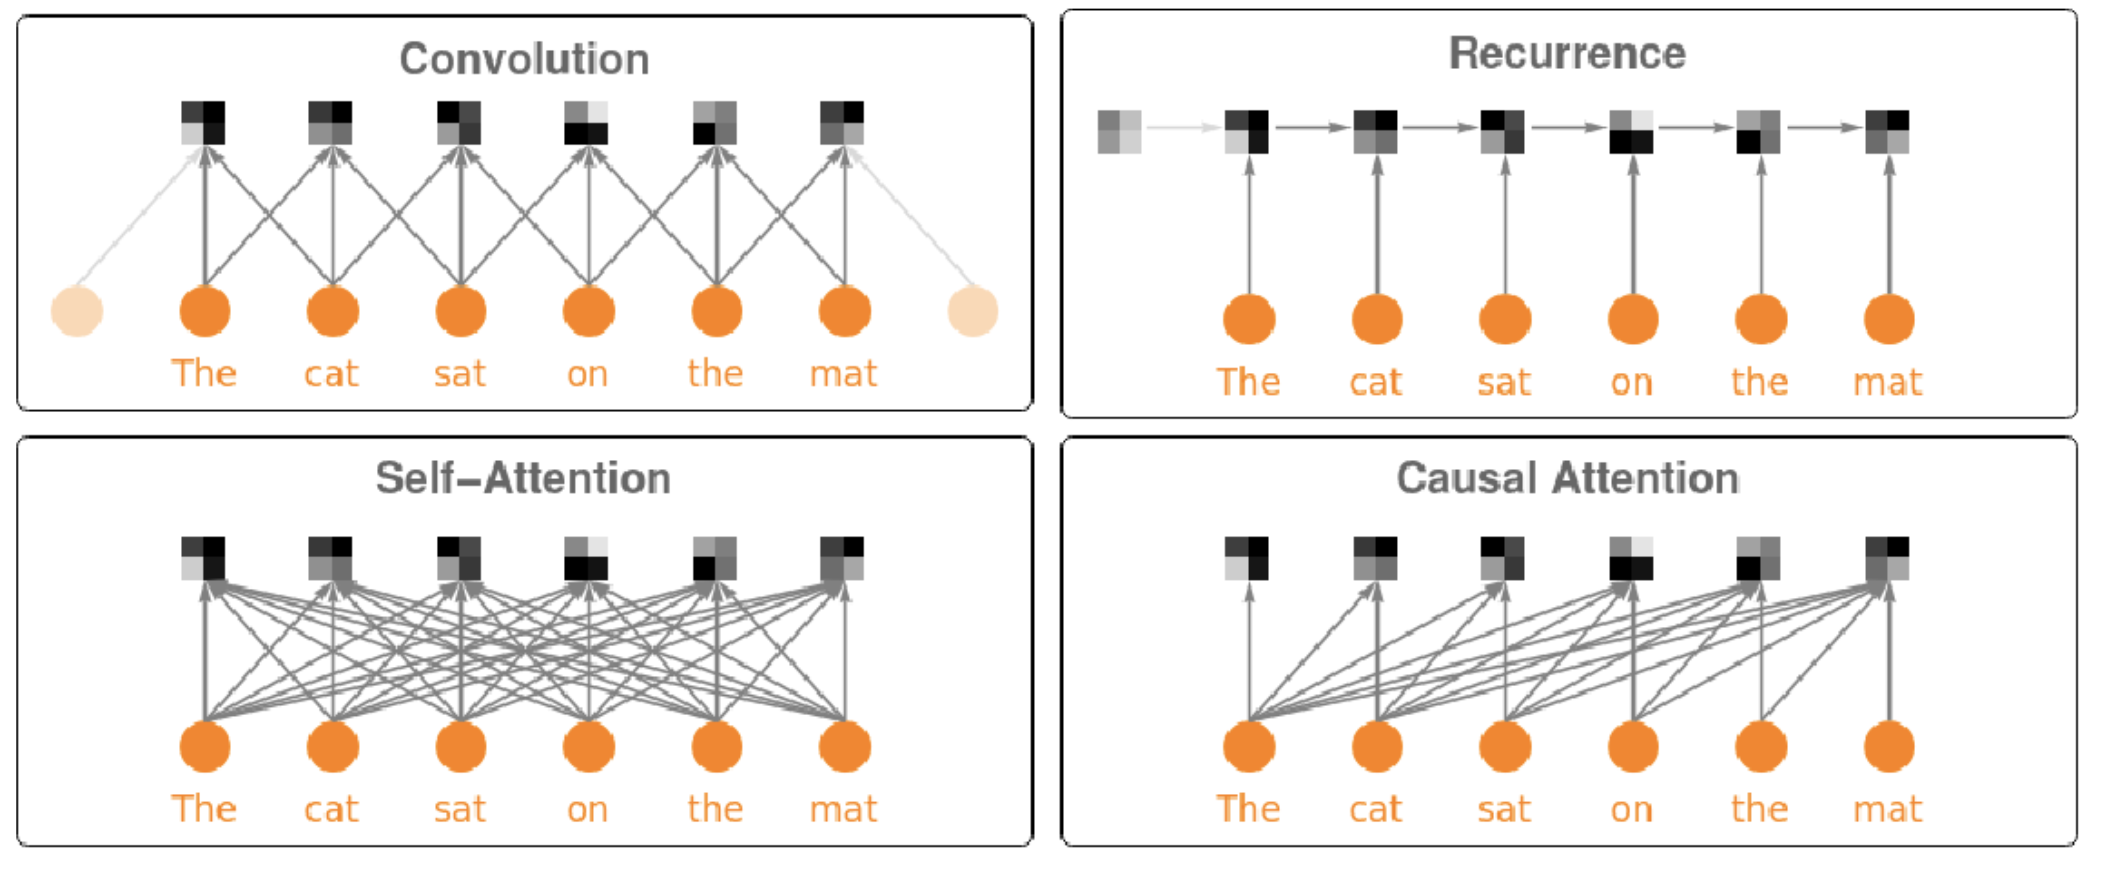
\includegraphics[width=0.7\textwidth]{figures/attention_graph.png}
  \end{center}
    \footnote{Image credit: \href{https://www.wolfram.com/language/12/neural-network-framework/use-transformer-neural-nets.html}{Wolfram.com}}
\end{frame}

\begin{frame}{Large Language Models}
\begin{itemize}
  \item Most LLMs today are large-scale decoder-only autoregressive (causal) Transformers (>1B parameters).
\end{itemize}
\begin{center}
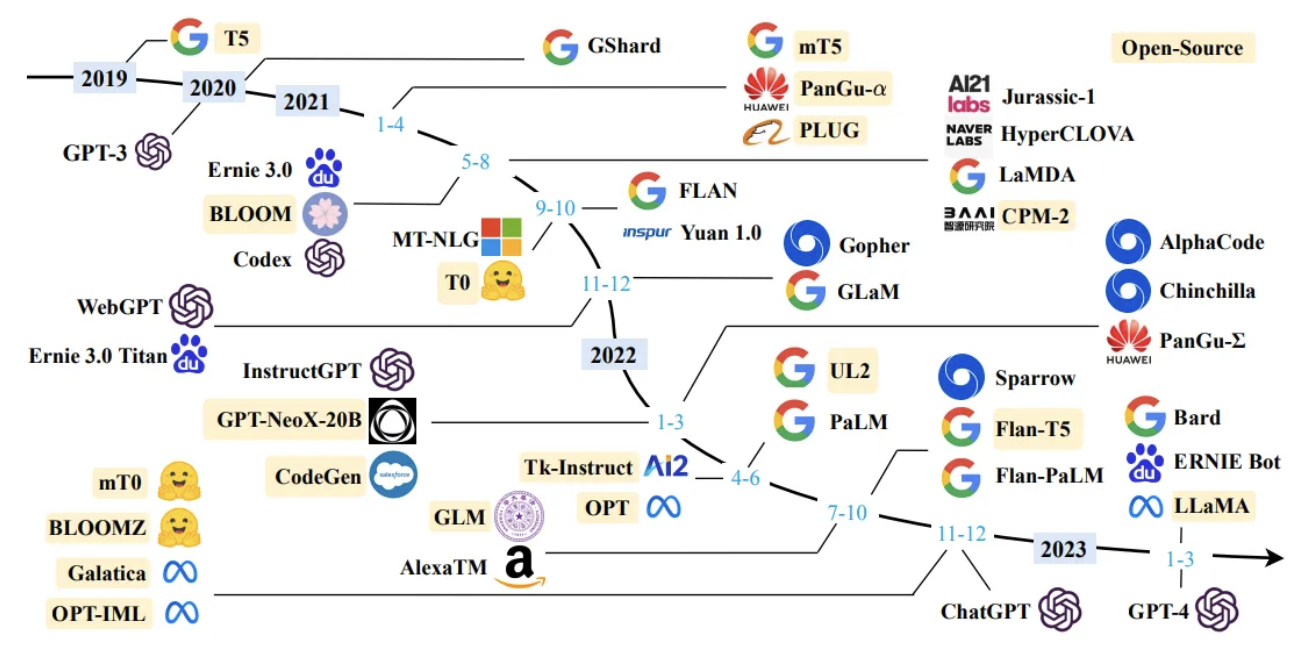
\includegraphics[width=0.7\textwidth]{figures/llm.png}
\footnote{Image credit: \href{https://medium.com/@thedatabeast/top-free-courses-on-large-language-models-abf2722d15c5}{Medium.com}}
\end{center}
\end{frame}

% \begin{frame}{Multi-modal learning}
% \end{frame}

% \begin{frame}{Visual attention}
% \end{frame}

% \begin{frame}{Visual question answering}
% \end{frame}

% \begin{frame}{Sequential attention}
% \end{frame}

% \begin{frame}{Instance segmentation with recurrent attention}
% \end{frame}

\begin{frame}{Interim Summary}
\begin{itemize}
  % \item A chunk of deep learning literature in the past 10 years focuses on better optimization, reduce overfitting, and architecture motifs.
  \item<+-> Optimization: Learning rate, initialization, activation functions, normalization, shortcut skip connection, attention, etc.
  \item<+-> Overfitting: Dropout, Data augmentation, etc.
  \item<+-> Architecture Motifs: MLP, CNN, RNN, Transformers, etc.
  \item<+-> Why it works? Data, optimization, compute.
  \item<+-> Still many open questions: Interpretability, fairness, uncertainty, data efficiency, energy efficiency, theory, etc.
\end{itemize}
\end{frame}

\section{Interpretability in Deep Neural Networks}

\begin{frame}{ML Interpretability}
\begin{itemize}
  \item<+-> Linear regression: Weights represent feature selection strength
  \item<+-> SVMs: Dual weights represent sample selection
  \item<+-> Bayesian methods: Model the generative process as a probabilistic model, fully transparent
  \item<+-> Decision trees: If-else decision making process
  \item<+-> Neural networks: ?
\end{itemize}
\end{frame}

\begin{frame}{Feature Visualization}
\begin{itemize}
  \item Recall: we can understand what first-layer features are doing by visualizing the weight matrices.
  \begin{center}
    \begin{columns}
      \begin{column}{0.35 \textwidth}
        \begin{center}
          Fully connected
          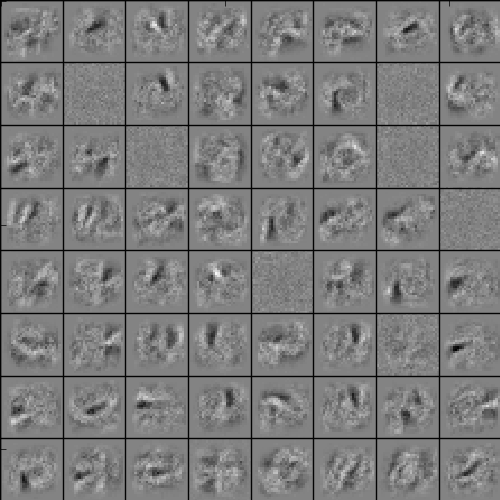
\includegraphics[width=0.6 \textwidth]{figures/mnist_filters.png}
        \end{center}
      \end{column}
      \begin{column}{0.35 \textwidth}
        \begin{center}
          Convolutional
          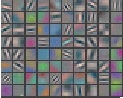
\includegraphics[width=0.55 \textwidth]{figures/zeiler_filters.pdf}
        \end{center}
        \begin{flushright}
  \tiny{Zeiler and Fergus, Visualizing and understanding convolutional networks, ECCV 2014.}
        \end{flushright}
      \end{column}
    \end{columns}
  \end{center}
\item The better the input matches these weights, the more the feature activates.
\item Higher-level weight matrices are hard to interpret.
\begin{itemize}
  \item Obvious generalization: visualize higher-level features by seeing what inputs activate them.
\end{itemize}
\end{itemize}
\end{frame}

\begin{frame}{Feature Visualization}
\begin{itemize}
\item One way to formalize: pick the images in the training set which activate a unit most strongly.
\item Here's the visualization for layer 1:
  \begin{center}
    \includegraphics[width=0.3 \textwidth]{figures/layer1.png}
  \end{center}
\end{itemize}
\begin{flushright}
  \tiny{Zeiler and Fergus, Visualizing and understanding convolutional networks, ECCV 2014.}
\end{flushright}
\end{frame}

\begin{frame}{Feature Visualization}
\begin{itemize}
\item Layer 3:
  \begin{center}
    \includegraphics[width=0.4 \textwidth]{figures/layer3.png}
  \end{center}
\end{itemize}
\begin{flushright}
  \tiny{Zeiler and Fergus, Visualizing and understanding convolutional networks, ECCV 2014.}
\end{flushright}
\end{frame}

\begin{frame}{Feature Visualization}
\begin{itemize}
\item Layer 4:
  \begin{center}
    \includegraphics[width=0.4 \textwidth]{figures/layer4.png}
  \end{center}
\end{itemize}
\begin{flushright}
  \tiny{Zeiler and Fergus, Visualizing and understanding convolutional networks, ECCV 2014.}
\end{flushright}
\end{frame}

\begin{frame}{Feature Visualization}
\begin{itemize}
\item Layer 5:
  \begin{center}
    \includegraphics[width=0.7 \textwidth]{figures/layer5.png}
  \end{center}
\end{itemize}
\begin{flushright}
  \tiny{Zeiler and Fergus, Visualizing and understanding convolutional networks, ECCV 2014.}
\end{flushright}
\end{frame}

\begin{frame}{Feature Visualization}
\begin{itemize}
  \item<+-> Higher layers seem to pick up more abstract, high-level information.
  \item<+-> Problems?
    \begin{itemize}
    \item<+->  Can't tell what the unit is actually responding to in the image.
    \item<+->  We may read too much into the results, e.g.~a unit may detect red, and the images that maximize its activation will all be stop signs.
    \end{itemize}
  \item<+-> Can use input gradients to diagnose what the unit is responding to.
\end{itemize}
\end{frame}

\begin{frame}{Feature Visualization}
\begin{itemize}
\item Input gradients can be hard to interpret.
\item Take a good object recognition conv net (Alex Net) and compute the gradient of $\log p(y= \textrm{``cat''} | \mathbf{x})$:
  \begin{center}
    \begin{columns}
      \begin{column}{0.35 \textwidth}
        \begin{center}
          Original image
          \includegraphics[width=0.8 \textwidth]{figures/cat.pdf}
        \end{center}
      \end{column}
      \begin{column}{0.35 \textwidth}
        \begin{center}
          Gradient for ``cat''
          \includegraphics[width=0.7 \textwidth]{figures/cat_gradient.pdf}
        \end{center}
      \end{column}
    \end{columns}
  \end{center}
\end{itemize}
\end{frame}

\begin{frame}{Feature Visualization}
  \begin{itemize}
  \item \alert{Guided backprop} is a total hack to prevent this cancellation.
  \item Do the backward pass as normal, but apply the ReLU nonlinearity to all the activation error signals.
    \[ y = \textrm{ReLU}(z) \qquad \bar{z} = \begin{cases} \bar{y} & \text{if $z > 0$ {\color{red} and $\bar{y} > 0$}} \\ 0 & \text{otherwise} \end{cases} \]
  \item We want to visualize what excites given unit, not what suppresses it.
    \begin{center}
      \includegraphics[width=0.5 \textwidth]{figures/guided_backprop_results.pdf}
    \end{center}
  \end{itemize}
\end{frame}

\begin{frame}{Guided Backprop}
\begin{center}
  \includegraphics[width=0.85 \textwidth]{figures/guided_backprop_results2.pdf}
\end{center}
\begin{flushright}
{\tiny Springerberg et al., Striving for simplicity: The all convolutional net, ICLR workshop 2015.}
\end{flushright}

% \notenew{
% \begin{itemize}
%   \item We start from here.
%   \item Visualize one neuron in the input image.
%   \item Draw one neuron in the middle.
% \end{itemize}
% }
\end{frame}


\begin{frame}{Class activation map (CAM)}

\begin{itemize}
\item Classification networks typically use global avg pooling before the final layer.

\item This pooling layer can already contain semantic information.

\item We can visualize a heat map 
\end{itemize}

\begin{center}
\includegraphics[height=0.3\textheight]{figures/cam.png}
\includegraphics[height=0.3\textheight]{figures/cam2.png}
\end{center}

\begin{flushright}
{\tiny Zhou et al. Learning deep features for discriminative localization. CVPR 2016.}
\end{flushright}

% \notenew{
%   \begin{itemize}
%     \item Another way is to think about the output classes.
%     \item Imagine you have a classifier.
%     \item What would be the region of the input that is responsible 
%     \item Utilize the average pooling layer.
%     \item Take the dot product between the activation at each location and the class vector
%   \end{itemize}
% }
\end{frame}

\begin{frame}{GradCAM}

\begin{center}
\vspace{-0.2in}
\includegraphics[width=0.7\textwidth]{figures/gradcam.png}
\includegraphics[width=0.45\textwidth,trim={0 0 16cm 0},clip]{figures/gradcam2.png}
\end{center}

\begin{flushright}
{\tiny Selvaraju et al. Grad-CAM: Visual explanations from deep networks via gradient-based localization. ICCV 2017.}
\end{flushright}

% \notenew{
%   \begin{itemize}
%     \item Potentially a way to combine guided backprop and CAM.
%     \item In the example, GBP is still plotting the dog, even though we are visualizing the cat neuron.
%     \item We can suppress it by overlapping it with CAM.
%   \end{itemize}
% }
\end{frame}


\begin{frame}{DeepDream\footnote{\href{https://blog.research.google/2015/07/deepdream-code-example-for-visualizing.html?m=1}{Google Research Blog}}}
\begin{itemize}
\item Start with an image, and run a conv net on it.
\item Change the image such that units which were already highly activated get activated even more strongly.
``Rich get richer.''
\end{itemize}
\begin{center}
  \hspace{-1em}\includegraphics[width=0.9\textwidth]{figures/deepdream1.pdf}
\end{center}

% \notenew{
% \begin{itemize}
%   \item What if we try to maximize all neuron in one layer at once?
% \end{itemize}
% }
\end{frame}

\begin{frame}{DeepDream}
\begin{center}
  \hspace{-1em}\includegraphics[width=0.9\textwidth]{figures/deepdream2.pdf}
\end{center}
\end{frame}

\begin{frame}{DeepDream}
\begin{center}
  \hspace{-1em}\includegraphics[width=0.7\textwidth]{figures/deepdream3.pdf}
\end{center}
\end{frame}

\begin{frame}{Gradient Ascent on Images}
\begin{itemize}
\item Doing gradient ascent on an image to maximize the activation of a given neuron.
  \begin{center}
    \hspace{-3em}\includegraphics[width=\textwidth]{figures/distill_gd.png}
  \end{center}
\end{itemize}
\begin{flushright}
  \begin{tiny}
    \vspace{-1em}
    \url{https://distill.pub/2017/feature-visualization/}
  \end{tiny}
\end{flushright}

% \notenew{
%   \begin{itemize}
%     \item Guided backpropagation = 1 step
%     \item What if we run multiple steps of gradients?
%   \end{itemize}
% }
\end{frame}

\begin{frame}{Gradient Ascent on Images}
\begin{center}
  \hspace{-1em}\includegraphics[width=\textwidth]{figures/distill_why_optimize.png}
\end{center}
\begin{flushright}
  \begin{tiny}
    \vspace{-1em}
    \url{https://distill.pub/2017/feature-visualization/}
  \end{tiny}
\end{flushright}

% \notenew{
%   \begin{itemize}
%     \item For the same layer, we can run it on different units, and get different results.
%     \item Above: dataset examples that maximizes neuron activation
%     \item Below: optimized images that maximizes neuron activation
%   \end{itemize}
% }
\end{frame}

\begin{frame}{Gradient Ascent on Images}
\begin{itemize}
  \item Higher layers in the network often learn higher-level, more interpretable representations
    \begin{center}
      \includegraphics[width=0.85 \linewidth]{figures/olah.png}
    \end{center}
    \begin{flushright}
      \begin{tiny}
        \vspace{-1em}
        \url{https://distill.pub/2017/feature-visualization/}
      \end{tiny}
    \end{flushright}
\end{itemize}
\end{frame}

\begin{frame}{Gradient Ascent on Images}
\begin{itemize}
  \item Higher layers in the network often learn higher-level, more interpretable representations
    \begin{center}
      \includegraphics[width=0.6 \linewidth]{figures/olah2.png}
    \end{center}
    \begin{flushright}
      \begin{tiny}
        \vspace{-1em}
        \url{https://distill.pub/2017/feature-visualization/}
      \end{tiny}
    \end{flushright}
\end{itemize}
\end{frame}


\begin{frame}{Artistic style transfer}
\begin{itemize}
\item Activation stores content information
\item Activation correlation across space stores style information and discards spatial arrangement
\end{itemize}
\begin{center}
\includegraphics[width=0.45\textwidth]{figures/style_transfer.png}
\end{center}
\begin{flushright}
{\tiny Gatys et al., Image style transfer Using convolutional neural networks, CVPR 2016.}
\end{flushright}

% \notenew{
%   \begin{itemize}
%     \item Backprop into the inputs can generate a lot of interesting patterns.
%     \item This could include low level image patterns.
%     \item What about change the style of an image?
%   \end{itemize}
% }
\end{frame}

\begin{frame}{Artistic style transfer}
\begin{itemize}
  \item Optimizing both content \& style from random noise
\end{itemize}
\begin{center}
\includegraphics[width=0.65\textwidth]{figures/style_transfer2.png}
\end{center}
\begin{flushright}
{\tiny Gatys et al., Image style transfer Using convolutional neural networks, CVPR 2016.}
\end{flushright}
\end{frame}

\begin{frame}{Artistic style transfer}
\begin{center}
\includegraphics[width=0.6\textwidth,trim={0 7cm 0 0},clip]{figures/style_transfer3.png}
\end{center}
\begin{flushright}
{\tiny Gatys et al., Image style transfer Using convolutional neural networks, CVPR 2016.}
\end{flushright}
\end{frame}

\begin{frame}{Adversarial Examples}
\begin{itemize}
\item One of the most surprising findings about neural nets has been the existence of \alert{adversarial inputs}, i.e.~inputs optimized to fool an algorithm.
\end{itemize}
\begin{center}
    \includegraphics[width=0.75 \linewidth]{figures/fgsm.png}
  \end{center}
\begin{flushright}
  \tiny{Goodfellow et al., Explaining and harnessing adversarial examples, ICLR 2015.}
\end{flushright}
% \notenew{
%     Given an image for one category (e.g.~``cat''), compute the image gradient to maximize the network's output unit for a different category (e.g.~``dog'')
%     \begin{itemize}
%       \item Perturb the image very slightly in this direction
%       \item Works slightly better if you take the sign of the entries in the gradient; this is called the \high{fast gradient sign method}.
%     \end{itemize}
% }
\end{frame}

\begin{frame}{Adversarial Examples}
\begin{itemize}
\item The following adversarial examples are misclassified as ostriches. ( $10 \times$ perturbation visualized in middle.)
  \begin{center}
    \includegraphics[width=0.85 \linewidth]{figures/adversarial_examples.png}
  \end{center}
\end{itemize}
\begin{flushright}
  \tiny{Szegedy et al., Intriguing properties of neural networks, ICLR 2014.}
\end{flushright}
\end{frame}

\begin{frame}{Adversarial Examples}
\begin{itemize}
\item You can print out an adversarial image and take a picture of it, and it still works!
  \begin{center}
    \includegraphics[width=0.9 \linewidth]{figures/printed_adversarial.png}
  \end{center}
  \begin{flushright}
    \tiny{Kurakin et al., Adversarial examples in the physical world, ICLR workshop 2017.}
  \end{flushright}
\end{itemize}
\end{frame}

\begin{frame}{Adversarial Examples}
\begin{itemize}
\item An adversarial example in the physical world (network thinks it's a gun, from a variety of viewing angles!)
  \begin{center}
    \includegraphics[width=0.7\textwidth]{figures/adversarial_physical.png}
  \end{center}
\end{itemize}
\begin{flushright}
  \tiny{Athalye et al., Synthesizing robust adversarial examples, ICML 2018.}
\end{flushright}
% \notenew{
%   \begin{itemize}
%   \item Optimize different view angles in 3D simulation, randomizing a lot of transformations.
%   \end{itemize}
% }
\end{frame}

\begin{frame}{Adversarial Examples}
\begin{itemize}
\item An adversarial mesh object that can hide cars from LiDAR detector
  \begin{center}
    \includegraphics[width=0.6\textwidth]{figures/adv_mesh.png}
  \end{center}
\end{itemize}
\begin{flushright}
  \tiny{Tu et al., Physically realizable adversarial examples for LiDAR object detection, CVPR 2020.}
\end{flushright}
% \notenew{
%   \begin{itemize}
%     \item People often use self-driving car as an example to emphasize the importance.
%     \item In this example, this is a 3D vision task, but the intuition is similar.
%     \item Tries to fool an object detector with a strange looking shape.
%   \end{itemize}
% }
\end{frame}

% \begin{frame}{Large Language Model Safety}
% \begin{itemize}
%   \item The vulnerability of deep networks also extend to LLMs.
%   \item People have recently come up with 
% \end{itemize}
% \end{frame}

\begin{frame}{Adversarial Defense}
\begin{itemize}
  \item How to defend from adversarial perturbation is still an active research area.
  \item Blackbox vs. whitebox attacks.
  \item One common approach is to train with millions of adversarial examples.
  \item Needs to train much longer, and also suffers a little from normal accuracy.
  \item Data augmentation and label smoothing also help.
\end{itemize}
% \notenew{
%   More to be covered in security \& privacy of deep learning.
% }
\end{frame}

\begin{frame}{Summary}
\begin{itemize}
  \item<+-> Interpretability - ways to open up the black box of neural networks
  \item<+-> Knowing what each neuron does is like studying a ``brain'' with perfect observation and measurement.
  \item<+-> Still very open research area.
  \item<+-> Adversarial examples are safety vulnerabilities of deep learning.
  \item<+-> Need more data and more robust learning objectives.
\end{itemize}
\end{frame}

\section{K-means Clustering}

\begin{frame}
{Unsupervised learning}
\begin{description}[<+->]
\item[Goal] Discover interesting \emph{structure} in the data.
\item[Formulation] Density estimation: $p(x;\theta)$ (often with \emph{latent} variables).
\item[Examples]
\begin{itemize}[<.->]
\item Discover \emph{clusters}: cluster data into groups.
\item Discover \emph{factors}: project high-dimensional data to a small number of ``meaningful'' dimensions, \ie dimensionality reduction.
\item Discover \emph{graph structures}: learn joint distribution of correlated variables, \ie graphical models.
\end{itemize}
\end{description}
\note[item]{Most of what we have learned so far belongs to supervised learning, where the core problem is to make predictions on unseen data given labeled training data. There is another important type of ML called unsupervised learning, where the main goal is to discover interesting patterns in the data.}
\note[item]{Unlike supervised learning, there is no obvious loss function since we don't know what patterns to look for. Instead, the problem is often formulated as density estimation where we aim to maximize the likelihood of the observed data.}
\note[item]{Clusters: group documents into different topics.}
\note[item]{Factors: variation among face images can be explained by a few factors such as illumination, pose, identity etc.}
\note[item]{Graph: phylogenetic tree of DNA evolution.}
\note[item]{We'll focus on clustering today.}
\end{frame}

\begin{frame}{Example: Old Faithful Geyser}
\includegraphics[height=0.6\textheight]{figures/oldfaithful}
\begin{itemize}
\item Looks like two clusters.
\item How to find these clusters algorithmically?
\end{itemize}
\note[item]{Let's consider a simple example. The old faithful geyser in Yellowstone has very predictable eruptions. It roughly erupts every 55 or 80 minutes. We can visualize this for 2D data, but how do we find these clusters more generally?}
\note[item]{One popular and simple algorithm is $k$-means. Let's go through the algorithm through this example.}
\end{frame}

\begin{frame}{$k$-Means: By Example}

\begin{itemize}
\item Standardize the data.
\item Choose two cluster centers.
\end{itemize}
\includegraphics[height=0.55\textheight]{{figures/faithful-9.1a}}

\let\thefootnote\relax\footnotetext{\tiny{From Bishop's \emph{Pattern recognition and machine learning}, Figure 9.1(a).}}
\note[item]{We first standardize the data and choose two points randomly. They will be the cluster center.}
\end{frame}

\begin{frame}{$k$-means: by example}

\begin{itemize}
\item Assign each point to closest center.
\end{itemize}
\includegraphics[height=0.55\textheight]{{figures/faithful-9.1b}}

\let\thefootnote\relax\footnotetext{\tiny{From Bishop's \emph{Pattern recognition and machine learning}, Figure 9.1(b).}}
\end{frame}
%
\begin{frame}{$k$-means: by example}

\begin{itemize}
\item Compute new cluster centers.
\end{itemize}
\includegraphics[height=0.55\textheight]{{figures/faithful-9.1c}}

\let\thefootnote\relax\footnotetext{\tiny{From Bishop's \emph{Pattern recognition and machine learning}, Figure 9.1(c).}}
\end{frame}
%
\begin{frame}{$k$-means: by example}

\begin{itemize}
\item Assign points to closest center.
\end{itemize}
\includegraphics[height=0.55\textheight]{{figures/faithful-9.1d}}

\let\thefootnote\relax\footnotetext{\tiny{From Bishop's \emph{Pattern recognition and machine learning}, Figure 9.1(d).}}
\end{frame}
%
\begin{frame}{$k$-means: by example}

\begin{itemize}
\item Compute cluster centers.
\end{itemize}
\includegraphics[height=0.55\textheight]{{figures/faithful-9.1e}}

\let\thefootnote\relax\footnotetext{\tiny{From Bishop's \emph{Pattern recognition and machine learning}, Figure 9.1(e).}}
\end{frame}
%
\begin{frame}{$k$-means: by example}

\begin{itemize}
\item Iterate until convergence.
\end{itemize}
\includegraphics[height=0.55\textheight]{{figures/faithful-9.1i}}

\let\thefootnote\relax\footnotetext{\tiny{From Bishop's \emph{Pattern recognition and machine learning}, Figure 9.1(i).}}
\note[item]{When do we achieve convergence? The cluster assignments no longer change.}
\note[item]{Does it always converge? Yes, more on this later.}
\note[item]{Does it always converge to good clusters? Not necessarily.}
\end{frame}

\begin{frame}{Suboptimal Local Minimum}

\begin{itemize}
\item The clustering for $k=3$ below is a local minimum, but suboptimal:
\end{itemize}
\includegraphics[width=0.8\textwidth]{figures/k-means-local-optimum}\let\thefootnote\relax\footnotetext{\tiny{From Sontag's DS-GA 1003, 2014, Lecture 8.}}
\note[item]{In this example, we have 3 clusters. But $k$-means found different cluster assignments than what we would do. It's a stationary point even though we can find ``better'' clusters.}
\note[item]{How do we define ``good'' clusters? Let's formalize $k$-means with an objective function.}
\end{frame}
%

\begin{frame}{Formalize $k$-Means}
\begin{itemize}[<+->]
\item Dataset $\cd=\left\{ x_{1},\ldots,x_{n}\right\} \subset\cx$ where $\sX = \reals^d$.

\item Goal: Partition data $\cd$ into $k$ disjoint sets $C_{1},\ldots,C_{k}$.
\item Let $c_i \in \pc{1, \ldots, k}$ be the cluster assignment of $x_i$.

\item The \textbf{centroid} of $C_{i}$ is defined to be
\begin{align}
\mu_{i}=\argmin_{\mu\in\cx}\sum_{x\in C_{i}}\|x - \mu\|^{2}.
&& \text{mean of $C_i$}
\end{align}

\item The $k$-means objective is to minimize the distance between each example and its cluster centroid:
\begin{align}
J(c, \mu) = \sum_{i=1}^n \| x_i - \mu_{c_i} \|^2 .
\end{align}
\end{itemize}
\note[item]{Define the centroid as the point that minimizes its distance to all other points in the cluster. In $\reals^d$,  the distance is Euclidean distance. If you solve this optimization problem, the centroid is the cluster mean.}
\end{frame}

%
\begin{frame}{$k$-Means: Algorithm}
\begin{enumerate}[<+->]
\item Initialize: Randomly choose initial centroids $\mu_{1},\ldots,\mu_{k} \in \reals^d$.

\item Repeat until convergence (i.e. $c_i$ doesn't change anymore):

\begin{enumerate}
\item For all $i$, set
\begin{align}
c_i \leftarrow \argmin_j \| x_i - \mu_j \|^2 .
&& \onslide<6->{\text{Minimize $J$ w.r.t. $c$ while fixing $\mu$}}
\end{align}

\item For all $j$, set 
\begin{align}
\mu_{j} \leftarrow \frac{1}{|C_j|}\sum_{x\in C_j} x .
&& \onslide<7->{\text{Minimze $J$ w.r.t. $\mu$ while fixing $c$.}}
\end{align}
\end{enumerate}
\end{enumerate}
\begin{itemize}
\item<5-> Recall the objective: $J(c, \mu) = \sum_{i=1}^n \| x_i - \mu_{c_i} \|^2$.
%\item<8-> $k$-means is coordinate descent on $J$.
\end{itemize}
\note[item]{Repeat two steps iteratively until convergence. 1) Assign points to their nearest cluster, where the distance is measured by the Euclidean distance between the point and the cluster centroid. 2) Update the cluster centroid given the assignments in the first step.}
\note[item]{Is this algorithm minimizing the objective?}
\note[item]{If we optimize the objective wrt each var while fixing other vars, what is it called?}
\end{frame}
%
\begin{frame}{Avoid bad local minima}
\begin{simpleblock}
{$k$-means converges to a local minimum.}
\begin{itemize}
%\item $k$-means is coordinate descent on $J$, thus $J$ will monotonically decrease.
\item $J$ is non-convex, thus no guarantee to converging to the global minimum.
\end{itemize}
\end{simpleblock}


\begin{simpleblock}
{Avoid getting stuck with bad local minima:}

\begin{itemize}[<+->]
\item Re-run with random initial centroids.
\item \textbf{$k$-means++}: choose initial centroids that spread over all data points.
\begin{itemize}[<+->] 
\item Randomly choose the first centroid from the data points $\cd$.
\item Sequentially choose subsequent centroids from points that are farther away from current centroids:
\begin{itemize}[<+->]
\item Compute distance between each $x_{i}$ and the closest already chosen
centroids.
\item Randomly choose next centroid with probability proportional to the
computed distance squared.
\end{itemize}
\end{itemize}
\end{itemize}
\end{simpleblock}

\note[item]{It can be shown that $k$-means++ converges to a solution not much worse than the optimal solution. Specifically, $\mathbb{E}\pb{J_{k\text{-means}++}} \le O(\log k) J^*$.}
\end{frame}

\begin{frame}
{Summary}
\begin{simpleblock}
{We've seen}
\begin{itemize}
\item Clustering---an unsupervised learning problem that aims to discover group assignments.
\item $k$-means:
\begin{itemize}
\item Algorithm: alternating between assigning points to clusters and computing cluster centroids.
\item Objective: minmizing some loss function by cooridinate descent.
\item Converge to a local minimum.
\end{itemize}
\end{itemize}
\end{simpleblock}

\onslide<2->{
\begin{simpleblock}
{Next, probabilistic model of clustering.}
\begin{itemize}
\item A generative model of $x$.
\item Maximum likelihood estimation.
\end{itemize}
\end{simpleblock}
}
\note[item]{At the beginning, we mentioned that unsupervised learning is often formulated as density estimation. But the $k$-means algorithm is not probabilistic. So next let's consider a probabilistic model of clustering and we will show that $k$-means is a special case of this approach.}
\end{frame}

\section{Gaussian Mixture Models}

\begin{frame}{Probabilistic Model for Clustering}
\onslide<1->{
\begin{columns}
\begin{column}{0.55\textwidth}
\begin{itemize}
\item Problem setup: 
\begin{itemize}
\item There are $k$ clusters (or \textbf{mixture components}).
\item We have a probability distribution for each cluster.
\end{itemize}
}

\onslide<2->{
\item Generative story of a \textbf{mixture distribution}:
\begin{enumerate}
\item Choose a random cluster $z\in\left\{ 1,2,\ldots,k\right\} $. 
\item Choose a point from the distribution for cluster $z$. 
\end{enumerate}
\end{itemize}
}
\end{column}

\onslide<3->{
\begin{column}{0.4\textwidth}
\begin{simpleblock}
{Example:}
\begin{enumerate}
\item Choose $z\in\left\{ 1,2,3\right\} $ with $p(1)=p(2)=p(3)=\frac{1}{3}$. 
\item Choose $x\mid z\sim\cn\left(X\mid\mu_{z},\Sigma_{z}\right)$.
\end{enumerate}
\end{simpleblock}

\includegraphics[height=0.5\textheight]{figures/mixture-3-gaussians}

\end{column}
}
\end{columns}
\note[item]{Remember that in probabilistic modeling, we want to model the distribution of $p(y\mid x)$ or $p(x, y)$. Here we don't have $y$, so let's model $p(x)$.}
    \note[item]{So what distribution family should we use to model $x$? Let's think about how $x$ may be generated. It is clear from the figure that there is a two step process. To generate a sample, first, we decide which cluster it comes from, then sample from a distribution of points in that cluster.}
\end{frame}

\begin{frame}
{Gaussian mixture model (GMM)}
\begin{simpleblock}
{Generative story of GMM with $k$ mixture components:}
\begin{enumerate}
\item Choose cluster $z\sim \text{Categorical}(\pi_1, \ldots, \pi_k)$.
\item Choose $x\mid z \sim \sN(\mu_z, \Sigma_z)$.
\end{enumerate}
\end{simpleblock}

\onslide<2->{
\begin{simpleblock}
{Probability density of $x$:}
\begin{itemize}
\item Sum over (marginalize) the \textbf{latent variable} $z$.
\end{itemize}
\begin{align}
\onslide<.->{p(x) &= \sum_z p(x, z) \\}
        \onslide<.->{&= \sum_z p(x\mid z) p(z) \\}
        \onslide<.->{&= \sum_k \pi_k \sN(\mu_k, \Sigma_k)}
\end{align}
\end{simpleblock}
}
\note[item]{How do we get the prob density of $x$? We know $p(x\mid z)$ and $p(z)$, which means that we know the joint distribution $p(x,z)$.}
\note[item]{Marginalization: expectation of conditional distribution: $\mathbb{E}_{Y}\pb{X\mid Y} = p(X)$.}
\end{frame}

\begin{frame}{Identifiability Issues for GMM}
\begin{itemize}
\item Suppose we have found parameters 
\begin{eqnarray*}
\text{Cluster probabilities}: &  & \pi=\left(\pi_{1},\ldots,\pi_{k}\right)\\
\text{Cluster means}: &  & \mu=\left(\mu_{1},\ldots,\mu_{k}\right)\\
\text{Cluster covariance matrices:} &  & \Sigma=\left(\Sigma_{1},\ldots\Sigma_{k}\right)
\end{eqnarray*}
 that are at a local minimum.
\end{itemize}

\pause{}
\begin{itemize}
\item What happens if we shuffle the clusters? e.g. Switch the labels for
clusters 1 and 2.
\end{itemize}

\pause{}
\begin{itemize}
\item We'll get the same likelihood. How many such equivalent settings are
there?
\end{itemize}

\pause{}
\begin{itemize}
\item Assuming all clusters are distinct, there are $k!$ equivalent solutions.
\end{itemize}

\pause{}
\begin{itemize}
\item Not a problem \emph{per se}, but something to be aware of.
\end{itemize}

    \note[item]{We should be careful when interpret the meaning of a cluster. It is tempting to say that cluster 1 is politics, 2 is sports etc. But we will always need to look at the examples in that cluster instead of just relying on the cluster id, which are interchangable.}
\end{frame}

\begin{frame}
{Learning GMMs}
\begin{simpleblock}
{How to learn the parameters $\pi_k, \mu_k, \Sigma_k$?}
\onslide<2->{
\begin{itemize}
\item MLE (also called maximize marginal likelihood).
\item Log likelihood of data:
\begin{align}
L(\theta) &= \sum_{i=1}^n \log p(x_i; \theta) \\
&= \sum_{i=1}^n {\color{red}\log \sum_z} p(x, z; \theta) 
\end{align}
}
\onslide<3->{
\item Cannot push $\log$ into the sum... $z$ and $x$ are coupled.
\item No closed-form solution for GMM---try to compute the gradient yourself!
}
\end{itemize}
\end{simpleblock}
\note[item]{Now that we have $p(x)$, how do we learn the parameters of the distribution?}
\note[item]{The log likelihood is just the log probability of the marginals, so it's also called MML when you have latent variables.}
\note[item]{The log sum term is annoying... That means that $z$ and $x$ are coupled and we probably don't have closed form solution. Recall that previously when we take derivative wrt some parameter $\theta_i$, we can ignore all terms whose subscript is not $i$ and the sums would be simplified.}
\end{frame}

\begin{frame}{Gradient Descent / SGD for GMM}
\begin{itemize}
\item What about running gradient descent or SGD on
\begin{eqnarray*}
J(\pi,\mu,\Sigma) & = & -\sum_{i=1}^{n}\log\left\{ \sum_{z=1}^{k}\pi_{z}\cn\left(x_{i}\mid\mu_{z},\Sigma_{z}\right)\right\} ?
\end{eqnarray*}


\pause{}
\item Can be done, in principle -- but need to be clever about it.

\pause{}
\item For example, each covariance matrix $\Sigma_{1},\ldots,\Sigma_{k}$ has to be positive semidefinite.

\pause{}
\item How to maintain that constraint?

\pause{}
\begin{itemize}
\item Rewrite $\Sigma_{i}=M_{i}M_{i}^{T}$, where $M_{i}$ is an unconstrained
matrix. 

\pause{}
\item Then $\Sigma_{i}$ is positive semidefinite. 

\pause{}
\end{itemize}
\item Even then, pure gradient-based methods have trouble.\footnote{See Hosseini and Sra's \href{https://arxiv.org/abs/1506.07677}{Manifold Optimization for Gaussian Mixture Models}
for discussion and further references.}
\end{itemize}
\end{frame}


\begin{frame}
{Learning GMMs: observable case}
\begin{simpleblock}
{Suppose we observe cluster assignments $z$. Then MLE is easy:}

\begin{align}
n_{z} &= \sum_{i=1}^{n}\ind{z_{i}=z}
&& \text{\# examples in each cluster}\\
\hat{\pi}(z) &= \frac{n_{z}}{n}
&& \text{fraction of examples in each cluster} \\
\hat{\mu}_{z} &= \frac{1}{n_{z}}\sum_{i:z_{i}=z}x_{i}
&& \text{empirical cluster mean} \\
\hat{\Sigma}_{z} &= \frac{1}{n_{z}}\sum_{i:z_{i}=z}\left(x_{i}-\hat{\mu}_{z}\right)\left(x_{i}-\hat{\mu}_{z}\right)^{T}.
&& \text{empirical cluster covariance}
\end{align}

\end{simpleblock}
\note[item]{Similar to Gaussian NB where cluster id is like the label of the example.}
\note[item]{How do we know $z$?}
\end{frame}

\begin{frame}
{Learning GMMs: inference}
\begin{simpleblock}
{The inference problem: observe $x$, want to know $z$.}
\begin{align}
\onslide<2->{p(z=j \mid x_i) &= p(x, z=j) / p(x) \\}
\onslide<3->{&= \frac{p(x\mid z=j)p(z=j)}{\sum_k p(x\mid z=k) p(z=k)} \\}
\onslide<4->{&= \frac{\pi_j \sN(x_i \mid \mu_j, \Sigma_j)}{\sum_k \pi_k \sN(x_i \mid \mu_k, \Sigma_k)}}
\end{align}
\end{simpleblock}
\onslide<5->{
\begin{itemize}
\item $p(z\mid x)$ is a \emph{soft assignment}.
\item If we know the parameters $\mu, \Sigma, \pi$, this would be easy to compute.
\end{itemize}
}
\note[item]{So now we are in a chicken and egg problem. If we know $z$, the parameters are easy to estimate. If we know the problems, $p(z\mid x)$ is easy to estimate.}
\end{frame}

\begin{frame}
{EM for GMM}
Let's compute the cluster assignments and the parameters iteratively.
\onslide<2->{
\begin{simpleblock}
{The expectation-minimization (EM) algorithm:}
\begin{enumerate}
\item Initialize parameters  $\mu, \Sigma, \pi$ randomly.
\item Run until convergence:
}
\begin{enumerate}
\onslide<3->{
\item E-step: fill in latent variables by inference.
\begin{itemize}
\item compute soft assignments $p(z\mid x_i)$ for all $i$.
\end{itemize}
}
\onslide<4->{
\item M-step: standard MLE for $\mu, \Sigma, \pi$ given ``observed'' variables.
\begin{itemize}
\item Equivalent to MLE in the observable case on data weighted by $p(z\mid x_i)$.
}
\end{itemize}
\end{enumerate}
\end{enumerate}
\end{simpleblock}
\end{frame}

\begin{frame}
{M-step for GMM}
\begin{itemize}
%\item {Recall the gradient is:}
%\begin{align}
%\frac{d }{d \theta} \sum_z \log p(x,z;\theta) = \mathbb{E}_{{\color{red}p(z\mid x)}} \pb{ \frac{d}{d\theta}{\color{blue}\log p(x, z)} } 
%\end{align}
\item Let $p(z\mid x)$ be the soft assignments:
\[
    \gamma_{i}^{j}=\frac{\pi_{j}^{\text{old}}\cn\left(x_{i}\mid\mu_{j}^{\text{old}},\Sigma_{j}^{\text{old}}\right)}{\sum_{c=1}^{k}\pi_{c}^{\text{old}}\cn\left(x_{i}\mid\mu_{c}^{\text{old}},\Sigma_{c}^{\text{old}}\right)} .
\]
\item \think{Exercise}: show that
\begin{eqnarray*}
    n_z &=& \sum_{i=1}^n \gamma_i^z \\
\mu_{z}^{\text{new}} & = & \frac{1}{n_{z}}\sum_{i=1}^{n}\gamma_{i}^{z}x_{i}\\
\Sigma_{z}^{\text{new}} & = & \frac{1}{n_{z}}\sum_{i=1}^{n}\gamma_{i}^{z}\left(x_{i}-\mu_{z}^{\text{new}}\right)\left(x_{i}-\mu_{z}^{\text{new}}\right)^{T}\\
\pi_{z}^{\text{new}} & = & \frac{n_{z}}{n} .
\end{eqnarray*}
\end{itemize}
\end{frame}

\begin{frame}{EM for GMM}

\begin{itemize}
\item Initialization
\end{itemize}
\includegraphics[height=0.55\textheight]{{figures/9.8a}}

\let\thefootnote\relax\footnotetext{\tiny{From Bishop's \emph{Pattern recognition and machine learning}, Figure 9.8.}}
\note[item]{Initially, we have two spherical Gaussian.}
\end{frame}
%
\begin{frame}{EM for GMM}

\begin{itemize}
\item First soft assignment:
\end{itemize}
\includegraphics[height=0.55\textheight]{{figures/9.8b}}

\let\thefootnote\relax\footnotetext{\tiny{From Bishop's \emph{Pattern recognition and machine learning}, Figure 9.8.}}
\note[item]{Then we do the soft assignments. The points have mixed cluster membership.}
\end{frame}
%
\begin{frame}{EM for GMM}

\begin{itemize}
\item First soft assignment:
\end{itemize}
\includegraphics[height=0.55\textheight]{{figures/9.8c}}

\let\thefootnote\relax\footnotetext{\tiny{From Bishop's \emph{Pattern recognition and machine learning}, Figure 9.8.}}
\note[item]{Re-estimate the Gaussians.}
\end{frame}
%
\begin{frame}{EM for GMM}

\begin{itemize}
\item After 5 rounds of EM:
\end{itemize}
\includegraphics[height=0.55\textheight]{{figures/9.8e}}

\let\thefootnote\relax\footnotetext{\tiny{From Bishop's \emph{Pattern recognition and machine learning}, Figure 9.8.}}

\end{frame}
%
\begin{frame}{EM for GMM}

\begin{itemize}
\item After 20 rounds of EM:
\end{itemize}
\includegraphics[height=0.55\textheight]{{figures/9.8f}}

\let\thefootnote\relax\footnotetext{\tiny{From Bishop's \emph{Pattern recognition and machine learning}, Figure 9.8.}}
\note[item]{Convergence: likelihood doesn't change much.}
\end{frame}

\begin{frame}
{EM for GMM: Summary}
\begin{itemize}
\item EM is a general algorithm for learning latent variable models.
\item \emph{Key idea}: if data was fully observed, then MLE is easy.
\begin{itemize}
\item E-step: fill in latent variables by computing $p(z\mid x, \theta)$.
\item M-step: standard MLE given fully observed data.
\end{itemize}
\item Simpler and more efficient than gradient methods.
\item Can prove that EM monotonically improves the likelihood and converges to a local minimum.
\item $k$-means is a special case of EM for GMM with \emph{hard assignments}, also called hard-EM.
\end{itemize}
\note[item]{$k$-means: covariance and cluster prior $\pi$ is fixed; only estimate $\mu$; posterior approximated by the delta function.}
\end{frame}

\section{Latent Variable Models }
\begin{frame}{General Latent Variable Model}
\begin{itemize}
\item Two sets of random variables: $z$ and $x$.
\item $z$ consists of unobserved \textbf{hidden variables}.
\item $x$ consists of \textbf{observed variables}.

\pause{}
\item Joint probability model parameterized by $\theta\in\Theta$:
\[
p(x,z\mid\theta)
\]
\end{itemize}

\pause{}
\begin{definition}
A\textbf{ latent variable model }is a probability model for which
certain variables are never observed.

\pause{}

\end{definition}

e.g. The Gaussian mixture model is a latent variable model.
\end{frame}

\begin{frame}{Complete and Incomplete Data}
\begin{itemize}
\item Suppose we observe some data $\left(x_{1},\ldots,x_{n}\right)$.

\pause{}
\item To simplify notation, take $x$ to represent the entire dataset
\[
x=\left(x_{1},\ldots,x_{n}\right),
\]
and $z$ to represent the corresponding unobserved variables
\[
z=\left(z_{1},\ldots,z_{n}\right).
\]
\item An observation of $x$ is called an \textbf{incomplete data set}.
\item An observation $\left(x,z\right)$ is called a \textbf{complete data
set}.
\end{itemize}
\end{frame}
%
 
\begin{frame}{Our Objectives}
\begin{itemize}
\item \textbf{Learning problem}: Given incomplete dataset $x$, find MLE
\[
\hat{\theta}=\argmax_{\theta}p(x\mid\theta).
\]


\pause{}
\item \textbf{Inference problem}: Given $x$, find conditional distribution
over $z$:
\[
p\left(z\mid x,\theta\right).
\]


\pause{}
\item For Gaussian mixture model, learning is hard, inference is easy.
\item For more complicated models, inference can also be hard. (See DSGA-1005)
\end{itemize}
\end{frame}
%
\begin{frame}{Log-Likelihood and Terminology}
\begin{itemize}
\item Note that
\[
\argmax_{\theta}p(x\mid\theta)=\argmax_{\theta}\left[\log p(x\mid\theta)\right].
\]


\pause{}
\item Often easier to work with this ``\textbf{log-likelihood}''.

\pause{}
\item We often call $p(x)$ the \textbf{marginal likelihood}, 
\begin{itemize}
\item because it is $p(x,z)$ with $z$ ``marginalized out'':
\[
p(x)=\sum_{z}p(x,z)
\]


\pause{}
\end{itemize}
\item We often call $p(x,z)$ the \textbf{joint}. (for ``joint distribution'')

\pause{}
\item Similarly, $\log p(x)$ is the \textbf{marginal log-likelihood}.
\end{itemize}
\end{frame}
%

\section{EM Algorithm}

\begin{frame}
    {Intuition}
    \head{Problem}: marginal log-likelihood $\log p(x;\theta)$ is hard to optimize (observing only $x$)

    \head{Observation}: complete data log-likelihood $\log p(x,z;\theta)$ is easy to optimize (observing both $x$ and $z$)

    \head{Idea}: guess a distribution of the latent variables $q(z)$ (soft assignments)

    Maximize the \textbf{expected complete data log-likelihood}:
    $$
    \max_\theta \sum_{z\in\sZ} q(z) \log p(x,z;\theta)
    $$

    \head{EM assumption}: the expected complete data log-likelihood is easy to optimize

    Why should this work?
\end{frame}

\section{Math Prerequisites}

\begin{frame}{Jensen's Inequality}

\begin{theorem}
[Jensen's Inequality]If $f:\reals\to\reals$ is a \textbf{convex}
function, and $x$ is a random variable, then
\[
\ex f(x)\ge f(\ex x).\pause
\]
Moreover, if $f$ is \textbf{strictly convex}, then equality implies
that $x=\ex x$ with probability $1$ (i.e. $x$ is a constant).
\end{theorem}


\pause{}
\begin{itemize}
\item e.g. $f(x)=x^{2}$ is convex. So $\ex x^{2}\ge\left(\ex x\right)^{2}$.
Thus 
\[
\var\left(x\right)=\ex x^{2}-\left(\ex x\right)^{2}\ge0.
\]
 
\end{itemize}
\end{frame}
%
\begin{frame}{Kullback-Leibler Divergence}

\begin{itemize}
\item Let $p(x)$ and $q(x)$ be probability mass functions (PMFs) on $\cx$. 
\item How can we measure how ``different'' $p$ and $q$ are?
\end{itemize}

\pause{}
\begin{itemize}
\item The \textbf{Kullback-Leibler} or \textbf{``KL'' Divergence} is defined
by
\begin{eqnarray*}
\kl(p\|q) & = & \sum_{x\in\cx}p(x)\log\frac{p(x)}{q(x)}.
\end{eqnarray*}
(Assumes $q(x)=0$ implies $p(x)=0$.)
\end{itemize}

\pause{}
\begin{itemize}
\item Can also write this as
\begin{eqnarray*}
\kl(p\|q) & = & \ex_{x\sim p}\log\frac{p(x)}{q(x)}.
\end{eqnarray*}
\end{itemize}
\end{frame}
%
\begin{frame}{Gibbs Inequality ($\kl(p\|q)\ge0$ and $\kl(p\|p)=0$)}
\begin{theorem}
[Gibbs Inequality]Let $p(x)$ and $q(x)$ be PMFs on $\cx$. Then
\[
\kl(p\|q)\ge0,
\]
with equality iff $p(x)=q(x)$ for all $x\in\cx$. 
\end{theorem}


\pause{}
\begin{itemize}
\item KL divergence measures the ``distance'' between distributions.
\end{itemize}

\pause{}
\begin{itemize}
\item Note:

\begin{itemize}
\item KL divergence \textbf{not a metric}.
\item KL divergence is \textbf{not symmetric}.
\end{itemize}
\end{itemize}
\end{frame}
%
\begin{frame}{Gibbs Inequality: Proof}

\begin{eqnarray*}
\kl(p\|q) & = & \ex_{p}\left[-\log\left(\frac{q(x)}{p(x)}\right)\right]\\
 \pause
 & \ge & -\log\left[\ex_{p}\left(\frac{q(x)}{p(x)}\right)\right]\mbox{\qquad\text{(Jensen's)}}\\
 \pause
 & = & -\log\left[\sum_{\left\{ x\mid p(x)>0\right\} }p(x)\frac{q(x)}{p(x)}\right]\\
 \pause
 & = & -\log\left[\sum_{x\in\cx}q(x)\right]\\
 \pause
 & = & -\log1=0.
\end{eqnarray*}


\pause{}
\begin{itemize}
\item Since $-\log$ is strictly convex, we have strict equality iff $q(x)/p(x)$
is a constant, which implies $q=p$ . 
\end{itemize}
\end{frame}

\section{The ELBO: Family of Lower Bounds on $\log p(x\mid\theta)$}
\begin{frame}{The Maximum Likelihood Estimator}

\includegraphics[width=0.85\textwidth]{figures/margLL-withMax.pdf}

    \note[item]{To give an overivew of the EM algorithm, let's use this 1-d illustration. The marginal log-likelihood is a complex non-convex function, and we would like to find the parameter  that maximizes the marginal log-likelihood. Because it's hard to directly maximize this function, we will maximize its lower bound instead. Now, there can be many possible lowerbounds, some are useless (example). The key of the EM algorithm is to construct "good" lowerbounds which are easy to optimize and tight, meaning if you optimize the lower bound you also optimize the true function.}
\end{frame}

\begin{frame}
    {Lower bound of the marginal log-likelihood}
    \begin{eqnarray*}
        \log p(x;\theta) & = & \log \sum_{z\in\sZ} p(x,z;\theta) \\
        \pause
        &=& \log \sum_{z\in\sZ} q(z) \frac{p(x,z;\theta)}{q(z)}\\
        \pause
        %\quad {\color{brown}= \log \BE_z\pb{p(x,z;\theta)}}\\
        &\ge& \sum_{z\in\sZ} q(z) \log \frac{p(x,z;\theta)}{q(z)}\\
        \pause
        %\quad {\color{brown}= \BE_z\pb{\log p(x,z;\theta)}} \\
        &\eqdef& \sL(q, \theta)
    \end{eqnarray*}
    \vspace{-2em}
    \begin{itemize}
        \setlength\itemsep{2pt}
        \item \textbf{Evidence}:  $\log p(x;\theta)$
        \item \textbf{Evidence lower bound (ELBO)}: $\sL(q, \theta)$
        \item $q$: chosen to be a family of tractable distributions
        \item Idea: \emph{maximize the ELBO} instead of $\log p(x;\theta)$
    \end{itemize}
\end{frame}

\begin{frame}{MLE, EM, and the ELBO}
\begin{itemize}
\item The MLE is defined as a maximum over $\theta$:
\[
\hat{\theta}_{\text{MLE}}=\argmax_{\theta}\left[\log p(x\mid\theta)\right].
\]
\item For any PMF $q(z)$, we have a lower bound on the marginal log-likelihood
\[
\log p(x\mid\theta)\ge\cl(q,\theta).
\]
\item In EM algorithm, we maximize the lower bound (ELBO) over $\theta$
and $q$:
\[
\hat{\theta}_{\text{EM}}\approx\argmax_{\theta}\left[\max_{q}\cl(q,\theta)\right]
\]
\end{itemize}

\pause{}
\begin{itemize}
\item In EM algorithm, $q$ ranges over all distributions on $z$.
\end{itemize}
\end{frame}

\begin{frame}{EM: Coordinate Ascent on Lower Bound}
\begin{itemize}
\item Choose sequence of $q$'s and $\theta$'s by ``\textbf{coordinate
ascent}'' on $\cl(q,\theta)$.

\pause{}
\item EM Algorithm (high level):
\begin{enumerate}
\item Choose initial $\theta^{\text{old}}$.
\item Let $q^{*}=\argmax_{q}\cl(q,\theta^{\text{old}})$

\pause{}
\item Let $\theta^{\text{new}}=\argmax_{\theta}\cl(q^{*},\theta)$.

\pause{}
\item Go to step 2, until converged.
\end{enumerate}
\item Will show:\textbf{ $p(x\mid\theta^{\text{new}})\ge p(x\mid\theta^{\text{old}})$}
\item \textbf{Get sequence of $\theta$'s with monotonically increasing
likelihood.}
\end{itemize}
\end{frame}

\begin{frame}{EM: Coordinate Ascent on Lower Bound}
\begin{center}
\includegraphics[height=0.5\textheight]{figures/EM-twosteps-Bishop9.14.png} 
\par\end{center}
\begin{enumerate}
\item Start at $\theta^{\text{old}}.$ 

\pause{}
\item Find $q$ giving best lower bound at $\theta^{\text{old}}$$\implies$
$\cl(q,\theta)$. 

\pause{}
\item $\theta^{\text{new}}=\argmax_{\theta}\cl(q,\theta)$.
\end{enumerate}
\let\thefootnote\relax\footnotetext{\tiny{From Bishop's \emph{Pattern recognition and machine learning}, Figure 9.14.}}
\end{frame}

\begin{frame}
    {Is ELBO a "good" lowerbound?}
    \begin{align*}
        \sL(q, \theta) &= \sum_{z\in\sZ} q(z) \log \frac{p(x,z \mid\theta)}{q(z)} \\
        &= \sum_{z\in\sZ} q(z)\log \frac{p(z\mid x,\theta)p(x\mid\theta)}{q(z)} \\
        &= -\sum_{z\in\sZ}q(z) \log \frac{q(z)}{p(z\mid x,\theta)}
        + \sum_{z\in\sZ} q(z) \log p(x\mid\theta) \\
        &= -\KL{q(z)}{p(z\mid x,\theta)} + \underbrace{\log p(x\mid\theta)}_{\text{evidence}}
    \end{align*}
    \vspace{-2em}
    \begin{itemize}
        \item \textbf{KL divergence}: measures ``distance'' between two distributions (not symmetric!)
        \item $\KL{q}{p}\ge 0$ with equality iff $q(z) = p(z\mid x)$.
        \item ELBO = evidence - KL $\le$ evidence
    \end{itemize}
\end{frame}

\begin{frame}{Maximizing over $q$ for fixed $\theta$.}
\begin{itemize}
\item Find $q$ maximizing
\begin{eqnarray*}
\cl(q,\theta) & = & -\kl[q(z),p(z\mid x,\theta)]+\underbrace{\log p(x\mid\theta)\pause}_{\text{no }q\text{ here}}
\end{eqnarray*}


\pause{}
\item Recall $\kl(p\|q)\ge0$, and $\kl(p\|p)=0$.

\pause{}
\item Best $q$ is $q^{*}(z)=p(z\mid x,\theta)$ and
\[
\pause\cl(q^{*},\theta)=-\underbrace{\kl[p(z\mid x,\theta),p(z\mid x,\theta)]}_{=0}+\log p(x\mid\theta)
\]


\pause{}
\item Summary:
\[
\log p(x\mid\theta)=\sup_{q}\cl(q,\theta)\qquad\forall\theta
\]
\item For any $\theta$, \textbf{sup is attained} at $q(z)=p(z\mid x,\theta)$. 
\end{itemize}
\end{frame}
%

%\begin{frame}
%    {\dis Justification for maximizing ELBO}
%    $
%    \sL(q, \theta) = -\KL{q(z)}{p(z\mid x;\theta)} + \log p(x;\theta)
%    $
%
%    Fix $\theta=\theta_0$ and $\max_q \sL(q, \theta_0)$: $q^* = p(z\mid x;\theta_0)$ 
%    \vspace{10em}
%
%    Let $\theta^*, q^*$ be the global optimzer of $\sL(q, \theta)$, then $\theta^*$ is the global optimizer of $\log p(x;\theta)$. (Proof: exercise)
%\end{frame}

\begin{frame}{Marginal Log-Likelihood \textbf{IS}\textbf{\textcolor{blue}{\LARGE{}
}}the Supremum over Lower Bounds}

\includegraphics[width=0.75\textwidth]{figures/sup-margLL.pdf} 
\end{frame}

\begin{frame}
    {Summary}
    \textbf{Latent variable models}: clustering, latent structure, missing lables etc.

    \head{Parameter estimation}: maximum marginal log-likelihood

    \head{Challenge}: directly maximize the \textbf{evidence} $\log p(x;\theta)$ is hard

    \head{Solution}: maximize the \textbf{evidence lower bound}:
    $$
    \text{ELBO} = \sL(q, \theta) = -\KL{q(z)}{p(z\mid x;\theta)} + \log p(x;\theta)
    $$

    \head{Why does it work?}
    \begin{align*}
        q^*(z) &= p(z\mid x; \theta) \quad \forall \theta \in \Theta \\
        \sL(q^*, \theta^*) &= \max_\theta \log p(x; \theta)
    \end{align*}
\end{frame}

\begin{frame}
    {EM algorithm}
    \emph{Coordinate ascent on $\sL(q, \theta)$}\\
    \begin{enumerate}
        \item Random initialization: $\theta^{\text{old}} \leftarrow \theta_0$
        \item Repeat until convergence
            \begin{enumerate}[(i)]
                \item $q(z) \leftarrow \argmax_q \sL(q, \theta^{\text{old}})$
                    \begin{align*}
                    \text{\textbf{Expectation} (the E-step):} \quad
                    q^*(z) &= p(z\mid x;\theta^{\text{old}}) \\
                        J(\theta) &= \sL(q^*, \theta) 
                    \end{align*}
                \item $\theta^{\text{new}} \leftarrow \argmax_\theta \sL(q^*, \theta)$
                    \begin{align*}
                        \text{\textbf{Maximization} (the M-step):} \quad
                        \theta^{\text{new}} \leftarrow \argmax_\theta J(\theta)
                    \end{align*}
            \end{enumerate}
    \end{enumerate}
\end{frame}

\begin{frame}{EM Algorithm}
\begin{enumerate}
%\item Choose initial $\theta^{\text{old}}$.
\item \textbf{Expectation Step}
\begin{itemize}
    \setlength\itemsep{1pt}
\item Let $q^{*}(z)=p(z\mid x,\theta^{\text{old}})$. {[}$q^{*}$ gives
best lower bound at $\theta^{\text{old}}${]}

\pause{}
\item Let
\[
J(\theta):=\cl(q^{*},\theta)=\underbrace{\sum_{z}q^{*}(z)\log\left(\frac{p(x,z\mid\theta)}{q^{*}(z)}\right)}_{\mbox{\textbf{expectation }w.r.t. }z\sim q^{*}(z)}
\]
 

\pause{}
\end{itemize}
\item \textbf{Maximization Step} 
\[
\theta^{\text{new}}=\argmax_{\theta}J(\theta).\pause
\]
{[}Equivalent to maximizing expected complete log-likelihood.{]}

\pause{}
%\item Go to step 2, until converged.
\end{enumerate}
        EM puts no constraint on $q$ in the E-step and assumes the M-step is easy.
        In general, both steps can be hard.
\end{frame}

\begin{frame}
    {Monotonically increasing likelihood}
    \begin{figure}
        \includegraphics[height=5cm]{figures/EM-twosteps-Bishop9.14.png}
    \end{figure}
    \vspace{-2em}
    Exercise: prove that EM increases the marginal likelihood monotonically
    $$
    \log p(x;\theta^{\text{new}}) \ge \log p(x;\theta^{\text{old}})
    \;.
    $$
    Does EM converge to a global maximum?

    \note[item]{$\log p(x, \theta_o) = \sL(q^*, \theta_o) \le \sL(q^*, \theta_n) \le \log p(x, \theta_n)$}
\end{frame}

\section{Variations on EM}

\begin{frame}{EM Gives Us Two New Problems}
\begin{itemize}
\item The ``E'' Step: Computing

\[
J(\theta):=\cl(q^{*},\theta)=\sum_{z}q^{*}(z)\log\left(\frac{p(x,z\mid\theta)}{q^{*}(z)}\right)
\]


\pause{}
\item The ``M'' Step: Computing
\[
\theta^{\text{new}}=\argmax_{\theta}J(\theta).\pause
\]


\pause{}
\item Either of these can be too hard to do in practice.
\end{itemize}
\end{frame}

\begin{frame}{Generalized EM (GEM)}
\begin{itemize}
\item Addresses the problem of a difficult ``M'' step.

\pause{}
\item Rather than finding 
\[
\theta^{\text{new}}=\argmax_{\theta}J(\theta),
\]
find \textbf{any} $\theta^{\mbox{new}}$ for which
\[
J(\theta^{\mbox{new}})>J(\theta^{\mbox{old}}).
\]


\pause{}
\item Can use a standard nonlinear optimization strategy
\begin{itemize}
\item e.g. take a gradient step on $J$.

\pause{}
\end{itemize}
\item We still get monotonically increasing likelihood. 
\end{itemize}
\end{frame}

\begin{frame}{EM and More General Variational Methods}
\begin{itemize}
\item Suppose ``E'' step is difficult:
\begin{itemize}
\item Hard to take expectation w.r.t. $q^{*}(z)=p(z\mid x,\theta^{\text{old}})$.
\end{itemize}

\pause{}
\item Solution: Restrict to distributions $\cq$ that are easy to work with. 

\pause{}
\item Lower bound now looser:
\[
q^{*}=\argmin_{q\in\cq}\kl[q(z),p(z\mid x,\theta^{\text{old}})]
\]
\end{itemize}
\end{frame}

% \begin{frame}{Deep Latent Variable Models}
% \end{frame}

% \begin{frame}{Variational Autoencoders}
% \end{frame}

% \begin{frame}{Vector Quantization (VQ)}
% \end{frame}

% \begin{frame}{Other Divergence Metrics}
% \end{frame}

% \begin{frame}{Diffusion Models}
% \end{frame}

\begin{frame}{Today's Summary}
\begin{itemize}
  \item Motivation: Unsupervised learning
  \item K-means: A simple algorithm for discovering clusters 
  \item Making k-means probabilistic: Gaussian mixture models
  \item More generally: Latent variable models
  \item Learning of latent variable models: EM
  \item Underlying principle: Maximizing ELBO
\end{itemize}
\end{frame}
\end{document}
